
\section*{\centering Summary}

The disequilibrium combination of abundant methane and carbon dioxide has been proposed as a promising exoplanet biosignature that is readily detectable with upcoming telescopes such as the James Webb Space Telescope. However, few studies have explored the possibility of non-biological CH$_4$ and CO$_2$ and related contextual clues. Here, we investigate whether magmatic volcanic outgassing on terrestrial planets can produce atmospheric CH$_4$ and CO$_2$ with a thermodynamic model. Our model suggests that volcanoes are unlikely to produce CH$_4$ fluxes comparable to biological fluxes. Improbable cases where volcanoes produce biological amounts of CH$_4$ also produce ample carbon monoxide. We show, using a photochemical model, that high abiotic CH$_4$ abundances produced by volcanoes would be accompanied by high CO abundances, which could be a detectable false positive diagnostic. Overall, when considering known mechanisms for generating abiotic CH$_4$ on terrestrial planets, we conclude that observations of atmospheric CH$_4$ with CO$_2$ are difficult to explain without the presence of biology when the CH$_4$ abundance implies a surface flux comparable to modern Earth's biological CH$_4$ flux. A small or negligible CO abundance strengthens the CH$_4$+CO$_2$ biosignature because life readily consumes atmospheric CO, while reducing volcanic gases likely cause CO to build up in a planet's atmosphere. Furthermore, the difficulty of volcanically-generated CH$_4$-rich atmospheres suitable for an origin of life may favor alternatives such as impact-induced reducing atmospheres.

\section{Introduction} \label{sec:intro}

Large telescopes will soon be used to search for biogenic waste gases in exoplanet atmospheres. Oxygen is the most extensively studied biosignature gas \citep{Meadows_2017,Meadows_2018}. Although many studies have proposed ways of identifying scenarios where non-living processes might mimic life by producing oxygen, i.e. false positives \citep{Domagal-Goldman_2014,Harman_2015,Luger_2015,Schwieterman_2019,Tian_2014,Wordsworth_2014}, the circumstances are unusual and contextual clues can distinguish abiotic scenarios \citep{Meadows_2018}.

However, even when life is present, oxygen biosignatures may be uncommon. Oxygenic photosynthesis is a complex metabolism that only evolved once on Earth \citep{Fischer_2016}. Additionally, oxygen was slow to accumulate in the Earth's atmosphere \citep{Lyons_2014}, and other planets may have low O$_2$ concentrations for billions of years despite having oxygenic photosynthetic life if there are large oxygen sinks \citep{Claire_2006}. Accumulation of oxygen may be especially challenging on planets orbiting M-dwarf stars due to their low visible photon flux, which potentially limits primary production \citep{Lehmer_2018}.

One alternative to detecting oxygen-rich planets like the modern Earth is to look for methane on planets like the Archean Earth. Before the rise of oxygen, methanogenic life could have sustained a methane-rich atmosphere, which could be detected with remote spectroscopy \citep{Kasting_2003,Schindler_2000}. 

Recently, \citet{KrissansenTotton_2018_diseq} proposed a criterion for methane biosignatures: finding abundant CH$_4$ in the presence of CO$_2$ (abbreviated CH$_4$+CO$_2$). This combination is compelling if the CH$_4$ mixing ratio is greater than 0.1\% because it is difficult to explain such an abundance with the short atmospheric lifetime of CH$_4$ in terrestrial atmospheres and non-biological methane sources such as serpentinization \citep{KrissansenTotton_2018_diseq}. This 0.1\% threshold value is for planets that orbit stars like the Sun and must be adjusted for different stellar types. For example, planets orbiting M-stars typically receive less near-UV radiation than planets orbiting Sun-like stars resulting in different photochemistry that promotes the build up of CH$_4$ \citep{Segura_2005,Grenfell_2007,Grenfell_2014,Rugheimer_2015,Rugheimer_2018}. \citet{KrissansenTotton_2018_diseq} argued that the CH$_4$ biosignature is strengthened by a low CO abundance because volcanoes that produce CH$_4$ should also likely generate CO. Additionally, living planets might have low CO because microbes consume CO \citep{Kharecha_2005}; coupled ecosystem-planetary models of the early Earth suggest atmospheric CO/CH$_4$ ratios declined dramatically with the emergence of chemoautotrophic ecosystems \citep{Sauterey_2020}.

Exploring false positives for methane biosignatures is timely. Biogenic O$_2$ or O$_3$ detections with upcoming telescopes such as the James Webb Space Telescope (JWST) will be extremely difficult \citep{Barstow_2016,KrissansenTotton_2018_detect,Lustig-Yaeger_2019,Wunderlich_2020,Fauchez_2019}, whereas CH$_4$+CO$_2$ biosignatures are more readily detectable. Indeed, an Archean-Earth like CH$_4$+CO$_2$ biosignature is potentially detectable on the planet TRAPPIST-1e with just 10 transits \citep{KrissansenTotton_2018_detect}. Thus, exploration of potential methane biosignature false positives and their contextual discriminants is needed.

The literature exploring false positives for methane biosignatures has primarily focused on CH$_4$ generation in deep-sea serpentinizing hydrothermal vents. \citet{Guzman-Marmolejo_2013} estimated a maximum CH$_4$ surface flux of 0.18 Tmol/yr ($6.8\times10^8$ molecules cm$^{-2}$ s$^-1$) from hydrothermal vents for planets with the same mass as Earth. Additionally, \citet{KrissansenTotton_2018_diseq} used Monte-Carlo simulations to estimate a probability distribution for maximum abiotic CH$_4$ production from this process. They suggest that $>$10 Tmol CH4/yr is highly unlikely. These estimated maximum fluxes are small compared to modern Earth's biological CH$_4$ flux of 30 Tmol/yr. 

However, investigations of abiotic CH$_4$ on Earth suggest that these estimates of abiotic CH$_4$ from hydrothermal vents are potentially unrealistically large. Serpentinization reactions involving water and ultramafic oceanic crust generate H$_2$ then, purportedly, H$_2$ might react with inorganic carbon in hydrothermal systems to generate CH$_4$. \citet{KrissansenTotton_2018_diseq} and \citet{Guzman-Marmolejo_2013} both estimated abiotic CH$_4$ fluxes assuming efficient reactions between H$_2$ and inorganic carbon. However, laboratory experiments have shown that, uncatalyzed, this reaction is extremely slow at hydrothermal vent temperatures and pressures preventing chemical equilibrium on timescales of at least months \citep{Reeves_2020}. Additionally, various lines of evidence suggest that much of the CH$_4$ observed in deep-sea hydrothermal vent waters is ultimately from biology \citep{Reeves_2020}. Furthermore, lifeless planets without silica-secreting organisms should have high ocean-water SiO$_2$ concentrations which suppresses the H$_2$, and therefore abiotic CH$_4$, produced from serpentinization \citep{Tutolo_2020}.

Impacts can likely generate abiotic CH$_4$ \citep{Zahnle_2020}, although impact-generated CH$_4$ is only probable early in a solar system's lifetime. The cratering record on the Moon shows that Earth's impact flux decreased dramatically by 3.5 Ga \citep{Marchi_2014}. Thus, extra solar systems that are several billion years old are probably unlikely to have abiotic CH$_4$ from this source.

Here, we investigate another potential false-positive for the CH$_4$+CO$_2$ biosignature: magma-sourced volcanic outgassing (i.e., not metamorphic). Negligible CH$_4$ has been observed in gases emitted by magmatic volcanoes on Earth \citep{Reeves_2020,Catling_2017}, although it has not been investigated whether substantial CH$_4$ is feasible for volcanoes in vastly different thermodynamic regimes. We simulate outgassing speciation for a range of magma temperatures, outgassing pressures, oxygen fugacities, volatile composition, and variable partitioning between subaerial and submarine volcanism. We examine whether volcanoes can produce CH$_4$ fluxes comparable to biological fluxes. Using a photochemical model we also investigate atmospheric composition of hypothetical planets with reducing volcanic gases to see whether volcanic CH$_4$ coincides with large atmospheric CO, which could be a detectable false positive marker. 

\section{Methods} \label{sec:methods}

\subsection{Model for calculating volcanic outgassing speciation} \label{sec:volcmodel}

Below, we describe our model for predicting the gases produced by an erupting mantle-sourced volcano. We follow \citet{Gaillard_2014} and solve for the gas-gas and gas-melt equilibrium in a C-O-H system. Our model differs from \citet{Gaillard_2014} because we do not consider nitrogen or sulfur species. Despite these differences, we obtain similar results to calculations made in \citet{Gaillard_2014}. We have also validated our code against the work of \citet{Liggins_2020} and \citet{Ortenzi_2020}, which have independently constructed similar outgassing models. Our Python code is published as an open-source software on the Github page https://github.com/Nicholaswogan/VolcGases. 

Figure \ref{fig:imagine} shows a highly schematic conceptualization of volcanic degassing typical of low-viscosity magma. Gas bubbles form in the magma when molecules like H$_2$O and CO$_2$ are exsolved. Within the gas bubbles, reactions drive the system to chemical equilibrium. The oxygen fugacity ($f_{\mathrm{O_2}}$) of the gas bubble is controlled by equilibrium with the oxygen fugacity of the magma \citep[e.g.][]{Kadoya_2020}. Gases bubbles are released from the magma and enter the overlying atmosphere or ocean.

\begin{figure*}
    \centering
    \includegraphics[width=\textwidth]{tex/3methane/figures/whole_thing_pretty_filled_v2.pdf}
    \caption{Qualitative sketch of degassing typical of low viscosity magma (e.g., Hawaiian volcanoes). Here, gas bubble reaches thermal and chemical equilibrium with a melt (no crystals are present). Note, degassing can occur in many different ways depending on magma viscosity and volatile content \citep{Gonnermann_2013}.}
    \label{fig:imagine}
\end{figure*}

\renewcommand{\arraystretch}{1.1}
\begin{table}
\caption{Model constants and variables}
\label{tab:1}
\centering
\begin{tabularx}{\textwidth}{l c c c >{\raggedright\arraybackslash}p{4.5cm}}
\hline \hline
&Constant or Variable & Value & Units & Definition   \\
\hline
\multirow{11}{*}{Constants}& $d_\mathrm{H_2O}$     & 2.3   & ...     & Solubility constant$^a$ \\
&$a_\mathrm{CO_2}$     & 1     & ...     & Solubility constant$^a$ \\
&$a_\mathrm{H_2O}$     & 0.54  & ...     & Solubility constant$^a$ \\
&$S_1$     & ... & ...     & Solubility constant$^a$ \\
&$S_2$     & ... & ...     & Solubility constant$^a$ \\
&$\mu_\mathrm{magma}$     & 64.52 & $\frac{\text{g magma}}{\text{mol magma}}$ & Molar mass of magma$^b$ \\
&$\mu_\mathrm{H_2O}$     & 18.02 & $\frac{\mathrm{g\:H_2O}}{\mathrm{mol\:H_2O}}$ & Molar mass of H$_2$O \\
&$\mu_\mathrm{CO_2}$     & 44.01 & $\frac{\mathrm{g\:CO_2}}{\mathrm{mol\:CO_2}}$ & Molar mass of CO$_2$ \\
&$K_1$     & $e^{-29755/T+6.55}$ & bar$^{0.5}$ & Equilibrium constant$^c$ \\
&$K_2$     & $e^{-33979/T+10.42}$     & bar$^{0.5}$ & Equilibrium constant$^c$ \\
&$K_3$     & $e^{-96444/T+0.22}$     & -     & Equilibrium constant$^c$ \\

\hline
\multirow{5}{*}{Input} &$P$&...& bar   & Total pressure of degassing \\
      &$T$      &...& K     & Temperature of magma and gas \\
      &$f_{\mathrm{O_2}}$      &...& bar   & Oxygen fugacity of the magma \\
      &$m_{\mathrm{CO_2}}^{\mathrm{tot}}$       &...& $\frac{\mathrm{g\:CO_2}}{\mathrm{g\:gas\:and\:magma}}$ & mass fraction CO$_2$ in magma before degassing \\
      &$m_{\mathrm{H_2O}}^{\mathrm{tot}}$       &...& $\frac{\mathrm{g\:H_2O}}{\mathrm{g\:gas\:and\:magma}}$ & mass fraction H$_2$O in magma before degassing \\\hline
\multirow{8}{*}{Output} & $x_{\mathrm{H_2O}}$      &...& $\frac{\mathrm{mol\:H_2O}}{\mathrm{mol\:magma}}$ & mol fraction of H$_2$O in the magma after degassing \\
      &$x_{\mathrm{CO_2}}$       &...& $\frac{\mathrm{mol\:CO_2}}{\mathrm{mol\:magma}}$ & mol fraction of CO$_2$ in the magma after degassing \\
      &$P_{\mathrm{H_2O}}$       &...& bar   & Partial pressure of H$_2$O \\
      &$P_{\mathrm{CO_2}}$       &...& bar   & Partial pressure of CO$_2$ \\
      &$P_{\mathrm{H_2}}$       &...& bar   & Partial pressure of H$_2$ \\
      &$P_{\mathrm{CO}}$       &...& bar   & Partial pressure of CO \\
      &$P_{\mathrm{CH_4}}$       &...& bar   & Partial pressure of CH$_4$ \\
      &$\alpha_{\mathrm{gas}}$       &...& $\frac{\mathrm{mol\:gas}}{\mathrm{mol\:gas\:and\:magma}}$ & mol fraction in gas phase \\
\hline
\multicolumn{5}{>{\raggedright\arraybackslash}p{\textwidth}}{
$^a$From \citet{Iacono-Marziano_2012}. See Appendix \ref{sec:solu_constants} to calculate $S_1$ and $S_2$.

$^b$Molar mass of Mt. Etna magma.

$^c$Calculated from the NASA thermodynamic database \citep{Burcat_2005}.}
\end{tabularx}
\end{table}

A mathematical model describes the volatiles in gas bubbles and magma. The amount of carbon and hydrogen that are exsolved by the magma into bubbles is governed by the solubility of CO$_2$ and H$_2$O, which we calculate with the solubility relations for mafic magmas described in \citet{Iacono-Marziano_2012}:
\begin{equation}\label{eq:solu1}
    \ln ({x_{{\text{C}}{{\text{O}}_{\text{2}}}}}) = {x_{{{\text{H}}_{\text{2}}}{\text{O}}}}{d_{{{\text{H}}_{\text{2}}}{\text{O}}}} + {a_{{\text{C}}{{\text{O}}_{\text{2}}}}}\ln ({P_{{\text{C}}{{\text{O}}_{\text{2}}}}}) + S_1
\end{equation}
\begin{equation}\label{eq:solu2}
    \ln ({x_{{{\text{H}}_{\text{2}}}{\text{O}}}}) = {a_{{{\text{H}}_{\text{2}}}{\text{O}}}}\ln ({P_{{{\text{H}}_{\text{2}}}{\text{O}}}}) + {S_1}
\end{equation}
Here, $x_\mathrm{CO_2}$ and $x_\mathrm{H_2O}$ are mol fractions of CO$_2$ and H$_2$O in the magma, respectfully. Additionally, $P_\mathrm{CO_2}$ and $P_\mathrm{H_2O}$ are the partial pressure of CO$_2$ and H$_2$O in gas bubbles suspended in the magma. The other terms in Equations \eqref{eq:solu1} and \eqref{eq:solu2} are solubility parameters with values shown in Table \ref{tab:1} except $S_1$ and $S_2$, which are further described in Appendix \ref{sec:solu_constants}. We use solubility relations appropriate for mafic magmas because rocky planets and moons in our solar system usually have basaltic crusts which suggests that mafic magma is common to most terrestrial bodies.

Volatile mol fractions (e.g., $x_\mathrm{H_2O}$) can be converted to mass fractions with the formula
\begin{equation} \label{eq:convert}
    {m_i} = \frac{{x_i}{\mu_i}}{\mu_\mathrm{magma}}
\end{equation}
Here, $m_i$ is mass fraction, $\mu_i$ is the volatile's molar mass, and $i$ can be either H$_2$O or CO$_2$. Table \ref{tab:1} gives the units of each term. 

We assume that after the hot gas exsolves from the magma into bubbles, it achieves thermodynamic equilibrium from the reactions
\begin{equation}
    {{\text{H}}_{\text{2}}}{\text{O}} \leftrightarrow {{\text{H}}_{\text{2}}}{\text{ + }}\frac{{\text{1}}}{{\text{2}}}{{\text{O}}_{\text{2}}}
\end{equation}
\begin{equation}
    {\text{C}}{{\text{O}}_{\text{2}}} \leftrightarrow {\text{CO + }}\frac{{\text{1}}}{{\text{2}}}{{\text{O}}_{\text{2}}}
\end{equation}
\begin{equation}
    {\text{C}}{{\text{O}}_{\text{2}}}{\text{ + 2}}{{\text{H}}_{\text{2}}}{\text{O}} \leftrightarrow {\text{C}}{{\text{H}}_{\text{4}}}{\text{ + 2}}{{\text{O}}_{\text{2}}}
\end{equation}
At thermodynamic equilibrium, the ratios of the fugacities of volatile species (denoted $f_i$) are related to the equilibrium constant corresponding to each chemical reaction. We assume that we can replace fugacities with partial pressures (denoted $P_i$). This approximation is reasonable for the temperatures and pressures involved in volcanic outgassing \citep{Holland_1984}. Thus,
\begin{equation}\label{eq:react1}
    {K_1} = \frac{{{f_{{{\text{H}}_2}}}f_{{{\text{O}}_{\text{2}}}}^{0.5}}}{{{f_{{{\text{H}}_{\text{2}}}{\text{O}}}}}} \approx \frac{{{P_{{{\text{H}}_2}}}f_{{{\text{O}}_{\text{2}}}}^{0.5}}}{{{P_{{{\text{H}}_{\text{2}}}{\text{O}}}}}}
\end{equation}
\begin{equation}\label{eq:react2}
    {K_2} = \frac{{{f_{{\text{CO}}}}f_{{{\text{O}}_2}}^{0.5}}}{{{f_{{\text{C}}{{\text{O}}_2}}}}} \approx \frac{{{P_{{\text{CO}}}}f_{{{\text{O}}_2}}^{0.5}}}{{{P_{{\text{C}}{{\text{O}}_2}}}}}
\end{equation}
\begin{equation}\label{eq:react3}
    {K_3} = \frac{{{f_{{\text{C}}{{\text{H}}_4}}}f_{{{\text{O}}_2}}^2}}{{{f_{{\text{C}}{{\text{O}}_2}}}f_{{{\text{H}}_2}{\text{O}}}^2}} \approx \frac{{{P_{{\text{C}}{{\text{H}}_4}}}f_{{{\text{O}}_2}}^2}}{{{P_{{\text{C}}{{\text{O}}_2}}}P_{{{\text{H}}_2}{\text{O}}}^2}} 
\end{equation}
We calculate equilibrium constants (e.g. $K_1$) using the NASA thermodynamic database \citep{Burcat_2005}. We assume that the gas is thermally and chemically coupled to the magma so that the oxygen fugacity ($f_\mathrm{O_2}$) of the gas is set by the oxygen fugacity of magma, as observed \citep{Symonds_1994}.  So far, we have 7 unknowns ($x_{\mathrm{CO_2}}$, $x_{\mathrm{H_2O}}$, $P_{\mathrm{CO_2}}$, $P_{\mathrm{H_2O}}$, $P_{\mathrm{CO}}$, $P_{\mathrm{H_2}}$, $P_{\mathrm{CH_4}}$) and only 5 equations. To close the system, we add three more equations and one more unknown. The first equation requires that the partial pressures sum to the total pressure:
\begin{equation}\label{eq:pres}
    {P_{{{\text{H}}_{\text{2}}}}} + {P_{{{\text{H}}_{\text{2}}}{\text{O}}}} + {P_{{\text{CO}}}} + {P_{{\text{C}}{{\text{O}}_{\text{2}}}}} + {P_{{\text{C}}{{\text{H}}_{\text{4}}}}} = P
\end{equation}
The final two equations are atom conservation equations for carbon and hydrogen:
\begin{equation}\label{eq:C_con}
    {\frac{{m_{{\text{C}}{{\text{O}}_{\text{2}}}}^{{\text{tot}}}}\mu_\mathrm{magma}}{{{\mu_{{\text{C}}{{\text{O}}_{\text{2}}}}}}}} = \frac{{{P_{{\text{C}}{{\text{O}}_{\text{2}}}}} + {P_{{\text{CO}}}} + {P_{{\text{C}}{{\text{H}}_{\text{4}}}}}}}{P}{\alpha _{{\text{gas}}}} + (1 - {\alpha _{{\text{gas}}}}){x_{{\text{C}}{{\text{O}}_{\text{2}}}}}
\end{equation}
\begin{equation}\label{eq:H_con}
    {\frac{{m_{{{\text{H}}_{\text{2}}}{\text{O}}}^{{\text{tot}}}}\mu_\mathrm{magma}}{{{\mu_{{{\text{H}}_2}{\text{O}}}}}}} = \frac{{{P_{{{\text{H}}_{\text{2}}}{\text{O}}}} + {P_{{{\text{H}}_{\text{2}}}}} + 2{P_{{\text{C}}{{\text{H}}_{\text{4}}}}}}}{P}{\alpha _{{\text{gas}}}} + (1 - {\alpha _{{\text{gas}}}}){x_{{{\text{H}}_{\text{2}}}{\text{O}}}}
\end{equation}
Equations \eqref{eq:C_con} and \eqref{eq:H_con} state that the total moles of either carbon or hydrogen should be equal to the moles of either element in the gas phase plus the moles in the magma. Here, $\alpha_\mathrm{gas}$ is the final unknown. It is the total moles in the gas phase divided by the total moles in the gas and magma combined. See Appendix \ref{sec:Derivation_con} for a full derivation of Equations \eqref{eq:C_con} and \eqref{eq:H_con}.

Given a gas and magma temperature ($T$), pressure ($P$),  oxygen fugacity ($f_{\mathrm{O_2}}$), and the total mass fraction (or mol fraction) of CO$_2$ and H$_2$O in the magma ($m_\mathrm{CO_2}^{\mathrm{tot}}$, and $m_\mathrm{H_2O}^{\mathrm{tot}}$), Equations \eqref{eq:solu1}, \eqref{eq:solu2}, \eqref{eq:react1} - \eqref{eq:H_con} are a system of 8 equations and 8 unknowns ($x_{\mathrm{CO_2}}$, $x_{\mathrm{H_2O}}$, $P_{\mathrm{CO_2}}$, $P_{\mathrm{H_2O}}$, $P_{\mathrm{CO}}$, $P_{\mathrm{H_2}}$, $P_{\mathrm{CH_4}}$,$\alpha_\mathrm{gas}$). We solve this system of equations numerically with the Scipy Python package.

The solution to this system of equilibrium equations provides an estimate of amount of each volatile species in gas bubbles in magma immediately before the gas leaves the magma. We assume bubbles remain in thermodynamic equilibrium with the surrounding melt until they are released into the overlying atmosphere or ocean, and volatile speciation does not continue evolve upon release. This does not exactly reflect real degassing. Observed outgassing chemistry suggest that volcanic gas re-equilibrates to temperatures slightly lower than the magma as the gas leaves the magma and is no longer chemically buffered by it \citep{Moussallam_2019,Kadoya_2020,Oppenheimer_2018}. We do not capture this complexity in the main text, although, in Appendix \ref{sec:kinetics} we investigate the closed system re-equilibration of volcanic gases and show that this process does not change our conclusions.

Once the unknowns are solved for, they can be used to calculate the gas production, i.e., the moles of gas produced per kilogram of magma erupted:
\begin{equation}\label{eq:production}
    q_i = 10^3\left(\frac{\alpha_\mathrm{gas}}{\mathrm{\mu_\mathrm{magma}}(1-\alpha_\mathrm{gas})}\right) \frac{P_i}{P}
\end{equation}
Here, $q_i$ is the gas production of species $i$ in mol gas/kg magma. Calculating $q_i$ is useful because it is related to the flux $F_i$ of gas $i$ to the atmosphere by the magma production rate:
\begin{equation}\label{eq:Flux}
    F_i=q_iQ_{m}
\end{equation}
Here, $Q_m$ is the magma production rate in kg magma/yr, and $F_i$ is in mol/yr. 

Several authors have shown that degassing can be affected by graphite saturation of magma \citep{Hirschmann_2008} or by the solubility of CO, CH$_4$, and H$_2$ in magma \citep{Wetzel_2013,Ardia_2013,Hirschmann_2012}. The gas speciation model described above does not account for these processes. However, in Appendix \ref{sec:graphite_sat} we introduce a more complex model that accounts for graphite saturation and CO, CH$_4$, and H$_2$ solubility, and show that this model produces very similar results to the simplified model described here.

\subsection{Monte-Carlo Simulations}\label{sec:monte}
We investigate volcanic false positives to the CH$_4$+CO$_2$ biosignature on two types of worlds: An Earth-like world with subaerial and submarine outgassing (Figure \ref{fig:digram}), and an ocean-world with only submarine outgassing. For each type of planet, we search for false positive scenarios by calculating volcanic outgassing speciation with a wide range of input parameters.

\begin{figure*}
    \centering
    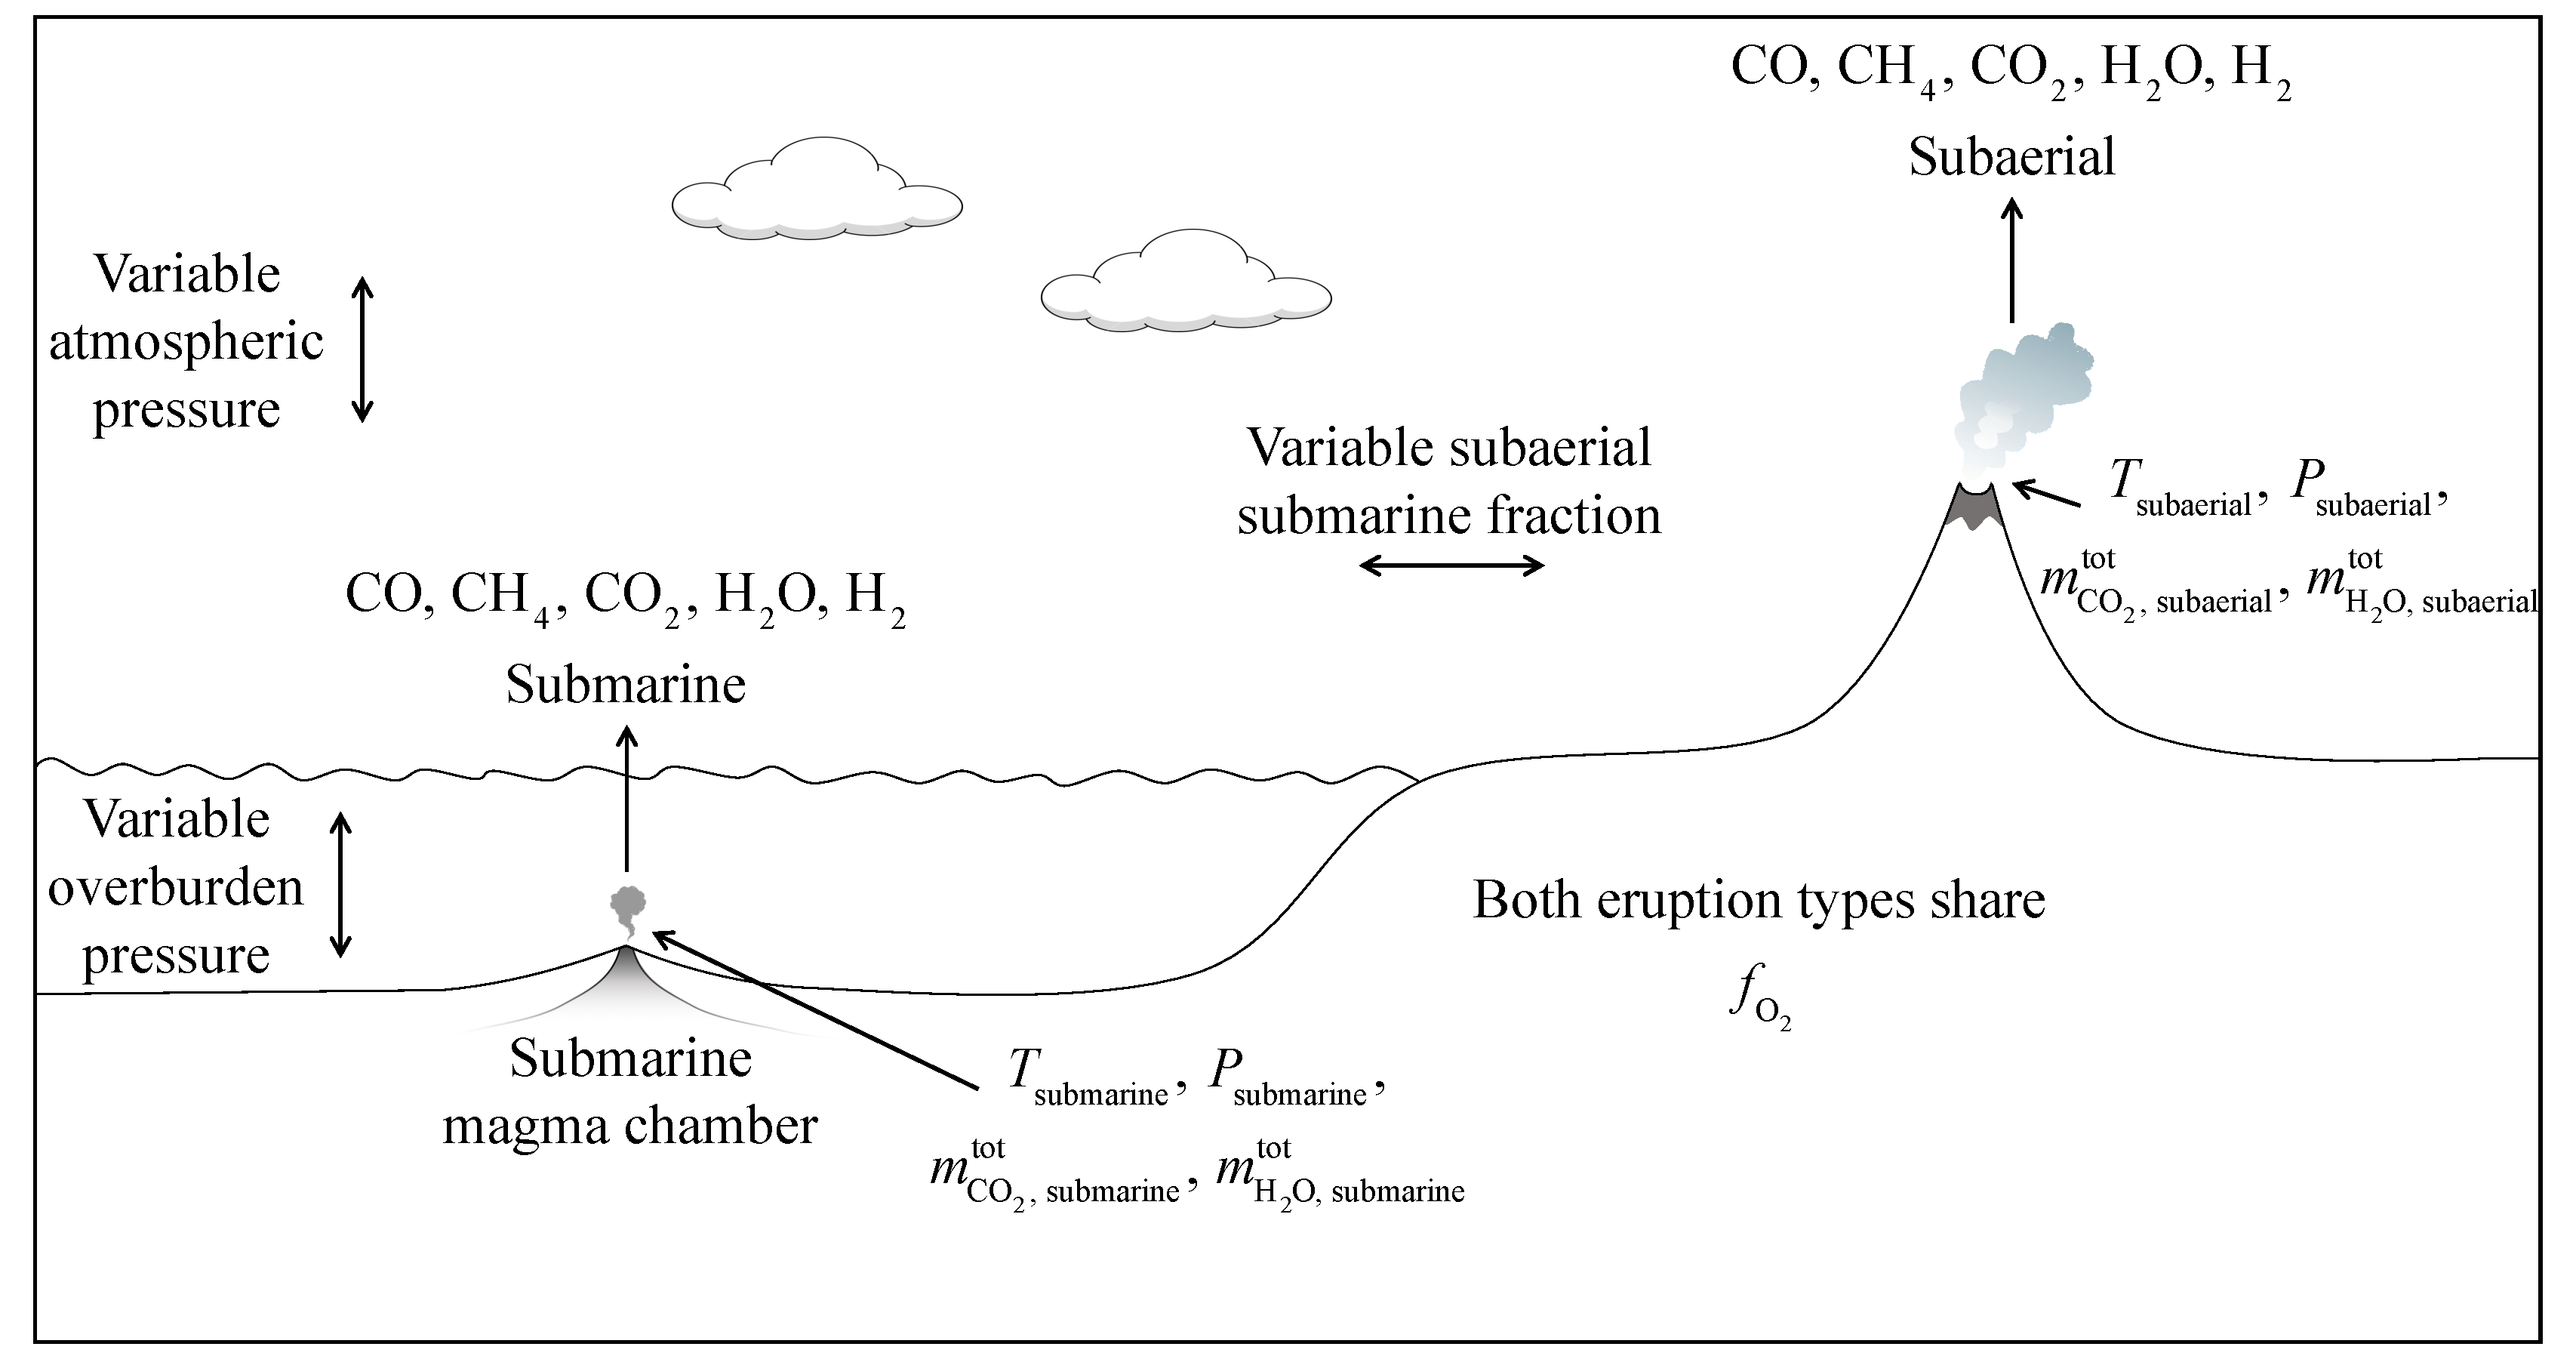
\includegraphics[width=\textwidth]{tex/3methane/figures/outgasing_diagram.pdf}
    \caption{Illustration of the parameters considered in the Monte-Carlo simulations.}
    \label{fig:digram}
\end{figure*}

\begin{table}
\caption{Monte-Carlo sampling distributions}
\label{tab:range}
\centering
\begin{tabularx}{0.95\linewidth}{p{0.15\linewidth} p{0.1\linewidth} p{0.1\linewidth} p{0.1\linewidth} p{0.4\linewidth}}
\hline \hline
  Variable & Low & High & Sampling method & Justification   \\
\hline
$T_\mathrm{submarine}$& 873 K & 1973 K   & linear uniform  & Range of submarine magma temperatures observed on Earth$^a$\\
$T_\mathrm{subaerial}$ & 873 K & 1973 K   & linear uniform  & Range of subaerial magma temperatures observed on Earth$^a$\\
$P_\mathrm{submarine}$ & 100 bar & 1000 bar  & linear uniform  & Degassing pressure at 1 km to 10 km ocean depth$^b$\\
$P_\mathrm{subaerial}$ & 0.001 bar & 100 bar  & log$_{10}$ uniform &    Rough range of subaerial degassing pressure in solar system \\
$m_\mathrm{CO_2,\:submarine}^\mathrm{tot}$ & $10^{-5}$ & $10^{-2}$ & log$_{10}$ uniform & Approx. CO$_2$ mass fraction range in Earth magma \citep{Wallace_2015,Wallace_2005,Anderson_2017,LeVoyer_2017} \\
$m_\mathrm{CO_2,\:subaerial}^\mathrm{tot}$ & $10^{-5}$ & $10^{-2}$   & log$_{10}$ uniform & Approx. CO$_2$ mass fraction range in Earth magma \citep{Wallace_2015,Wallace_2005,Anderson_2017,LeVoyer_2017}\\
$m_\mathrm{H_2O,\:submarine}^\mathrm{tot}$ & $10^{-5}$ & $10^{-1}$   & log$_{10}$ uniform & H$_2$O mass fraction range for Earth submarine outgassing \citep{Wallace_2015} \\
$m_\mathrm{H_2O,\:subaerial}^\mathrm{tot}$ & $10^{-5}$ & $10^{-1}$   & log$_{10}$ uniform & H$_2$O mass fraction range for Earth subaerial outgassing \citep{Wallace_2015} \\
$f_\mathrm{O_2}$ & FMQ-4 & FMQ+5   & log$_{10}$ uniform & Oxygen fugacity of most reducing Martian meteorite \citep{Catling_2017} to most oxidized magma on Earth \citep{Stamper_2014}$^c$ \\
$X$ & 0     & 1   & linear uniform & 0\% to 100\% subaerial volcanism\\
\hline
\multicolumn{5}{>{\raggedright\arraybackslash}p{\textwidth}}{
$^a$Coldest rhyolite magma, and hottest komatiites magmas \citep{Huppert_1984}

$^b$Assumes Earth's gravity. The solubility of H$_2$O in magma does not allow for significant CH$_4$ degassing at pressures greater than 1000 bar, equivalent to a depth of 10 km. 

$^c$FMQ is the fayalite-magnetite-quartz mineral redox buffer. See Chapter 7 in \citet{Catling_2017} for a description of mineral redox buffers. We use the parameterization for the FMQ buffer defined by \citet{Wones_1969}. This parameterization has only been experimentally validated to 1400 K \citep{ONeill_1987}, but we extrapolate using the parameterization to 1973 K}.
\end{tabularx}
\end{table}

To explore volcanism on Earth-like planets, we calculate outgassing speciation 10,000 times. For each calculation, we sample either uniform or log$_{10}$-uniform distributions (See Table \ref{tab:range}) of 10 parameters: $T_\mathrm{submarine}$, $P_\mathrm{submarine}$, $m_\mathrm{CO_2, \:\mathrm{submarine}}^{\mathrm{tot}}$, $m_\mathrm{H_2O, \:\mathrm{submarine}}^{\mathrm{tot}}$, $T_\mathrm{subaerial}$, $P_\mathrm{subaerial}$, $m_\mathrm{CO_2,\: \mathrm{subaerial}}^{\mathrm{tot}}$, $m_\mathrm{H_2O,\: \mathrm{subaerial}}^{\mathrm{tot}}$, $f_\mathrm{O_2}$, and $X$ . The width of each uniform sampling distribution are given and explained in Table \ref{tab:range}. We use inputs with subscripts “subaerial” to calculate subaerial volcanic speciation and inputs with subscripts “submarine” to calculate submarine volcanic speciation, and then we combine the results of each calculation with the formula
\begin{equation}
    {n_i} = \frac{{{P_{i{\text{, subaerial}}}}}}{{{P_{\text{subaerial}}}}}X + \frac{{{P_{i{\text{, submarine}}}}}}{{{P_{\text{submarine}}}}}(1 - X)
\end{equation}
Here, $n_i$ is the mixing ratio of averaged outgassed volatiles of species $i$ produced by the combination of subaerial and submarine volcanoes and $X$ is the fraction of subaerial volcanism ($0<X<1$). Also, $P_{i,\mathrm{\:subaerial}}$ and $P_{i,\mathrm{\: submarine}}$ are the partial pressure of species $i$ in subaerial and submarine outgassing, respectively.

To investigate volcanism on an ocean-world, we also calculate outgassing speciation 10,000 times. For each calculation, we sample either uniform or log$_{10}$-uniform distributions of inputs $T_\text{submarine}$, $P_\text{submarine}$ , $m_\mathrm{CO_2, \text{ submarine}}^{\mathrm{tot}}$, $m_\mathrm{H_2O, \text{ submarine}}^{\mathrm{tot}}$, and $f_\mathrm{O_2}$ with ranges defined and justified in Table \ref{tab:range}.

\subsection{Photochemical modeling: Uninhabited anoxic ocean-world with reducing volcanic gases}\label{method:photo}
We further investigate the CH$_4$+CO$_2$ biosignature by modeling the atmospheric composition of hypothetical uninhabited ocean-worlds with reducing volcanic gases. We consider planets orbiting the Sun, and a late M star - the latter because planets orbiting M-dwarfs are the most feasible targets for near-term telescopes like JWST \citep{Barstow_2016}.	Additionally, we simulate ocean-worlds because ocean-bottom degassing is most thermodynamically prone to produce CH$_4$, as revealed by our Monte-Carlo simulations and previous studies \citep{Kasting1998,French_1966} (see Section \ref{sec:water_solu} for further discussion).

To simulate atmospheres on uninhabited planets, we use the 1-D photochemical model contained within the open source software package \textit{Atmos}. \textit{Atmos} is derived from a model originally developed by the Kasting group \citep{Pavlov_2001}, and versions of this code have been used to simulate the Archean and Proterozoic Earth atmosphere \citep{Zahnle_2006}, Mars \citep{Sholes_2019,Smith_2014,Zahnle_2008}, and exoplanet atmospheres \citep{Harman_2015,Schwieterman_2019}. 

\section{Results}

\subsection{Monte-Carlo simulations}
\begin{figure*}
  \centering
  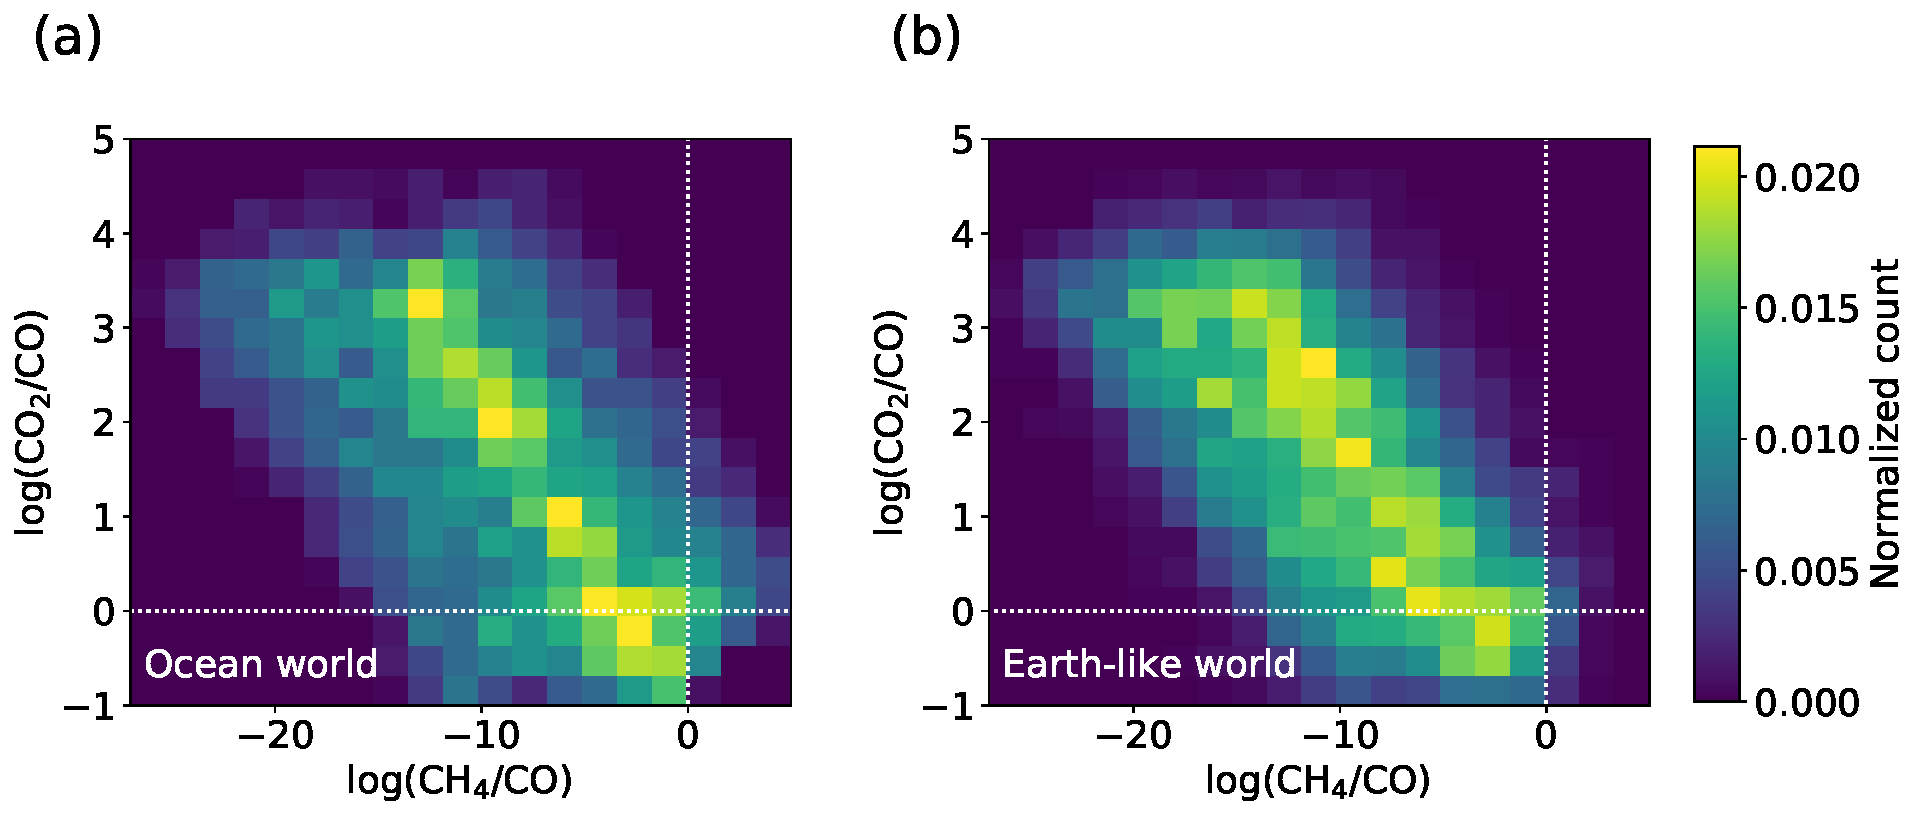
\includegraphics[width=\textwidth]{tex/3methane/figures/both.pdf}
  \caption{Results of the Monte-Carlo simulation described in Section 2.2. (a) and (b) show normalized count as a function of $\log(\mathrm{CH_4/CO})$ and $\log(\mathrm{CO_2/CO})$ for an ocean world and Earth-like world, respectively. The white dotted lines indicate where CH$_4$/CO = 1 and CO$_2$/CO = 1. For almost all calculated gas speciations, CO$_2$ and CO are much more abundant than CH$_4$.}
  \label{fig:result1}
\end{figure*}

Figure \ref{fig:result1} shows joint distributions of gas ratios CH$_4$/CO and CO$_2$/CO from the Monte-Carlo simulation described in Section \ref{sec:monte}. These results suggest that for most combinations of parameters volcanoes are most likely to produce more CO$_2$ than CO, and negligible CH$_4$, which is the case for the modern Earth \citep{Catling_2017}. About 7\% and 2\% of calculations produce more CH$_4$ than CO for ocean worlds and Earth-like worlds, respectfully. In the vast majority of cases, either CO or CO$_2$ is the dominant carbon-bearing species.

Figure \ref{fig:CH4}a and \ref{fig:CH4}b show CH$_4$ production from the Monte-Carlo simulations in terms of mol CH$_4$/kg magma. To give a sense for the gas fluxes implied by these CH$_4$ productions, we multiply the distributions in Figure \ref{fig:CH4}a and \ref{fig:CH4}b by the magma production rate of modern Earth of $9\times10^{13}$ kg/yr \citep{Crisp_1984}, which gives the gas fluxes shown in Figure \ref{fig:CH4}c and \ref{fig:CH4}d, respectively. About 0.1\% of calculations predict more than 10 Tmol CH$_4$/yr for both Earth-like worlds and ocean worlds. This small fraction suggests that for modern Earth magma production rates, volcanoes are unlikely to produce CH$_4$ fluxes comparable to modern Earth's biological flux of 30 Tmol/yr \citep{Hauglustaine_2007}.

Magma production rates larger than modern Earth's increase the probability that volcanic fluxes of CH$_4$ become comparable to biological CH$_4$ fluxes. For example, the early Archean Earth could have had magma production rates up to about 25 times modern Earth's \citep{Sleep_2001}. Such a magma production rate would shift the distributions in Figure \ref{fig:CH4}c and \ref{fig:CH4}d to larger values by a factor of 25 (or in log$_{10}$-space, by a factor of 1.4). In this case, $\sim$2\% of calculations (for either Earth-like world or ocean world) would predict more than 10 Tmol CH$_4$/yr. 

Crucially, large CH$_4$ fluxes should almost always coincide with even larger CO fluxes (horizontal axis in Figure \ref{fig:result1}). Therefore, the unlikely cases where volcanoes mimic biological CH$_4$ fluxes can be identified by detecting abundant CO in a planet's atmosphere. We further investigate CO as a CH$_4$+CO$_2$ biosignature discriminant using a photochemical model in the following section.

\begin{figure*}
  \centering
  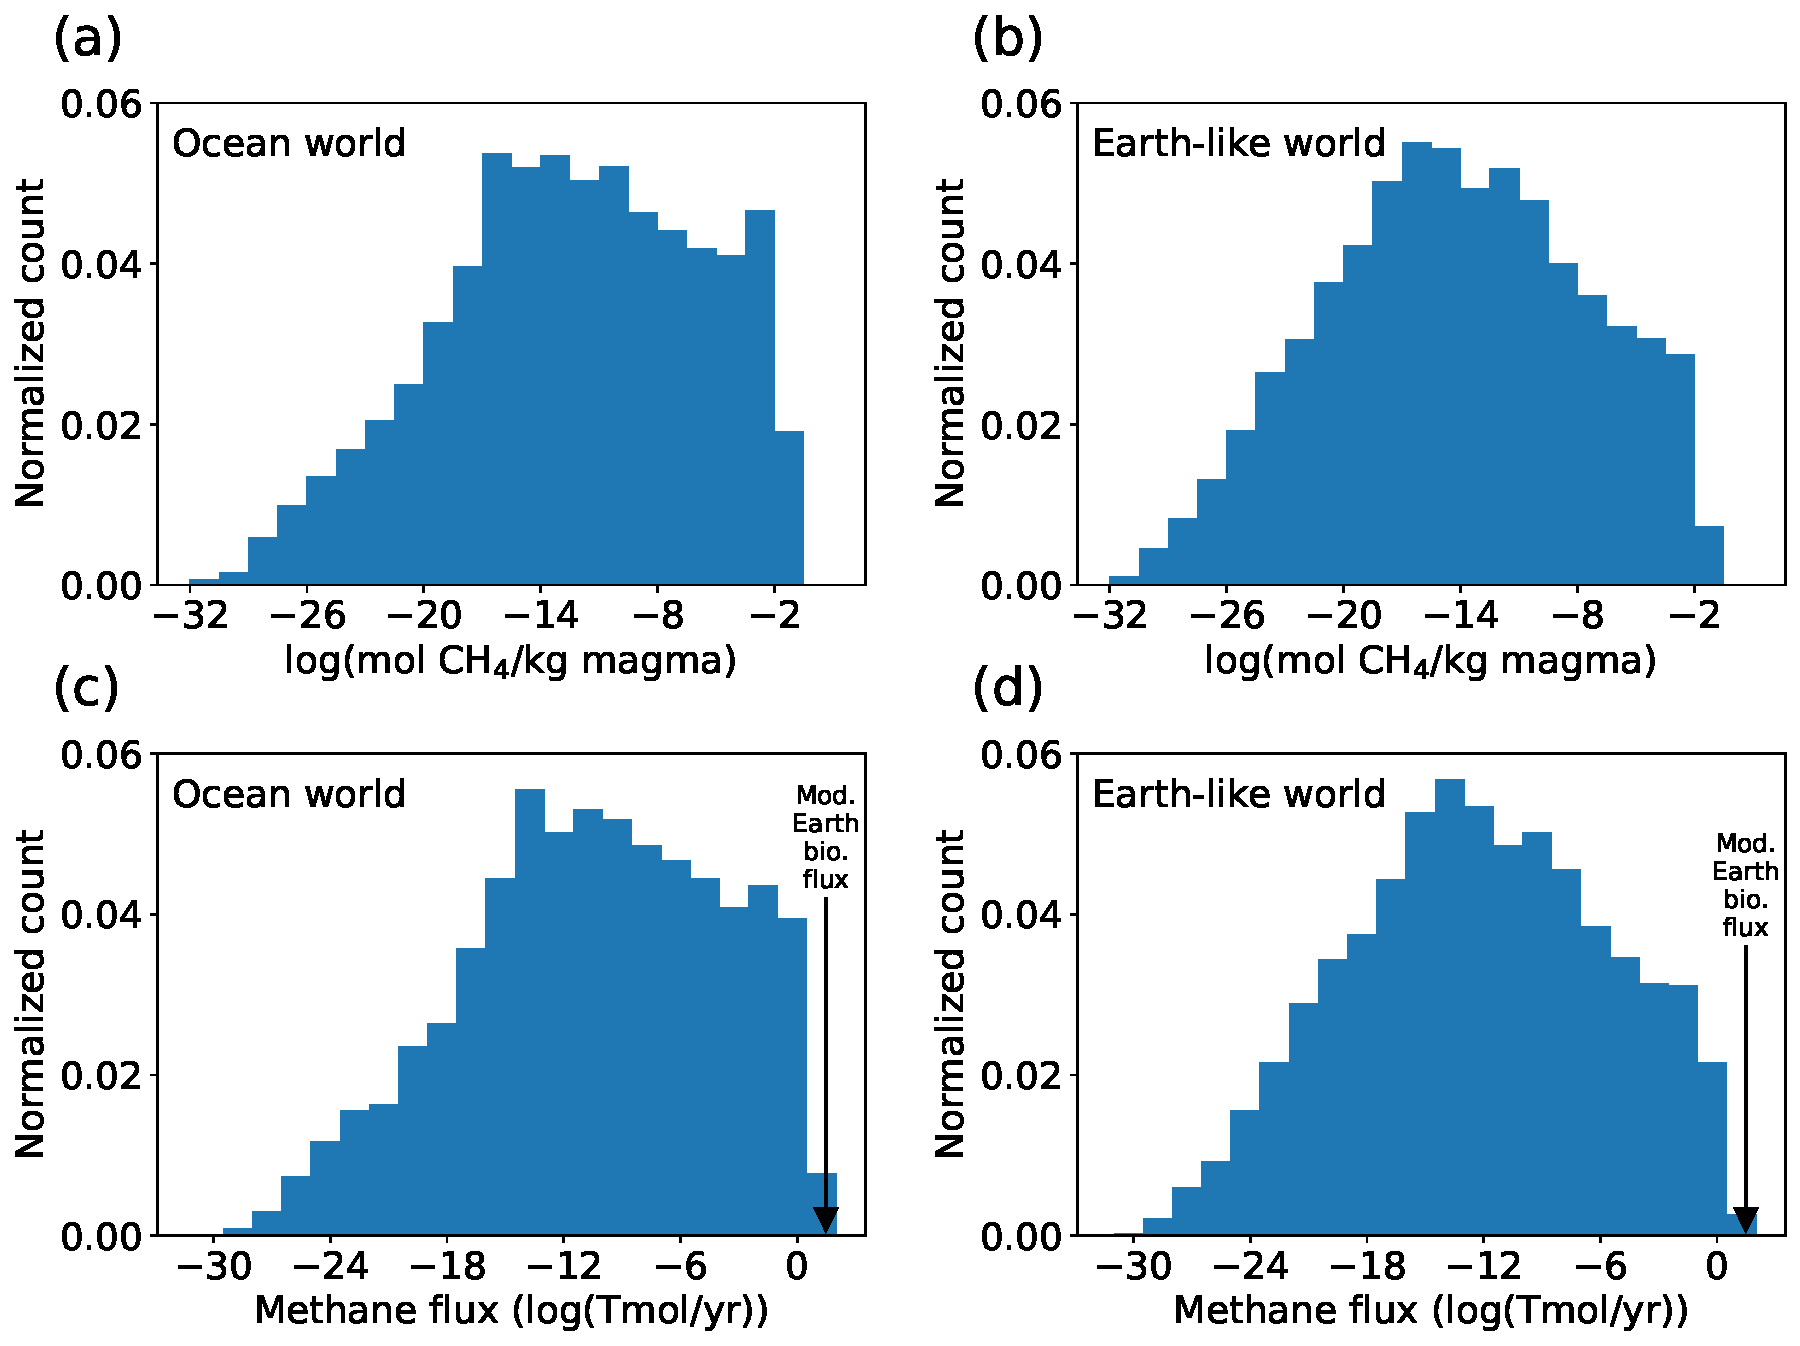
\includegraphics[width=\textwidth]{tex/3methane/figures/CH4_prod.pdf}
  \caption{Normalized count of methane production (mol gas/kg magma) for (a) ocean worlds and (b) Earth-like worlds. Distributions were calculated by sampling the ranges in Table \ref{tab:range}. Multiplying Earth's magma production rate of $9\times10^{13}$ kg magma/yr by (a) and (b) gives the methane fluxes in (c) and (d), respectively. For modern Earth's magma production rate, volcanoes are likely to produce negligible CH$_4$.}
  \label{fig:CH4}
\end{figure*}

\subsection{Photochemical modeling: Uninhabited anoxic ocean-world with reducing volcanic gases}\label{sec:photochem}

\begin{figure*}
  \centering
  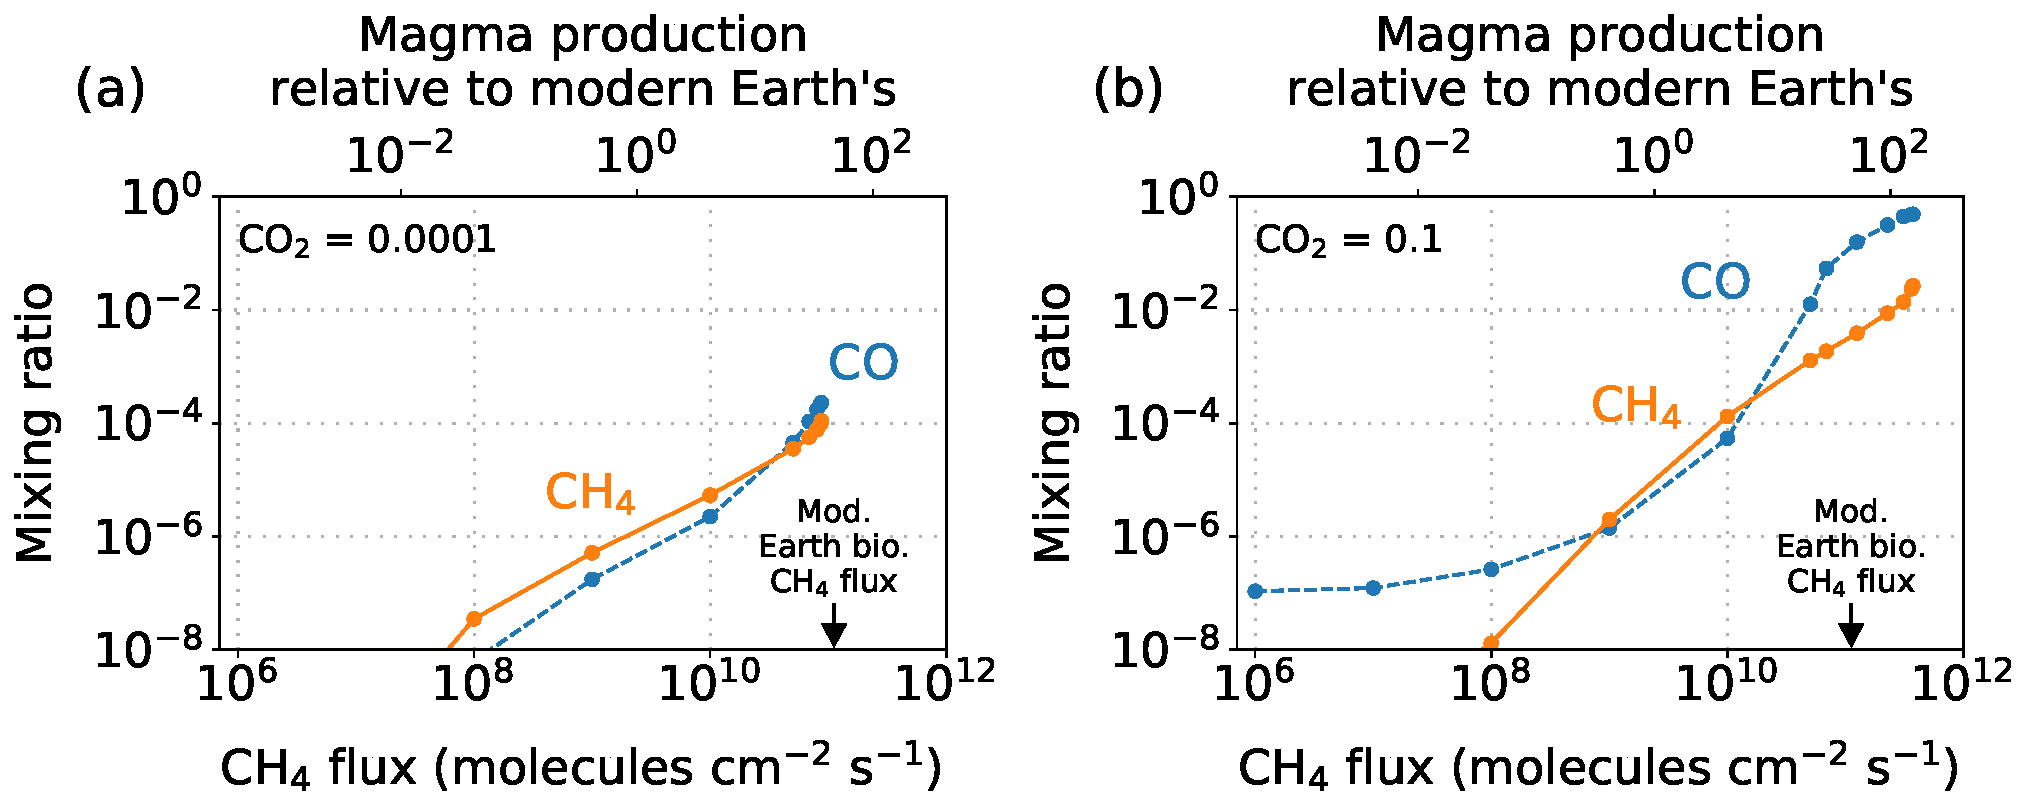
\includegraphics[width=\textwidth]{tex/3methane/figures/Figure4.pdf}
  \caption{Atmospheric mixing ratios of CO and CH$_4$ as a function of magma production rate relative to modern Earth's (or CH$_4$ flux) on an anoxic ocean-world with reducing volcanic gases orbiting a sun-like star. (a) and (b) are identical model runs, except (a) assumes a constant atmospheric CO$_2$ mixing ratio of 0.0001, and (b) assumes a constant atmospheric CO$_2$ mixing ratio of 0.1. Modern Earth's biological CH$_4$ flux is indicated on the horizontal axes. Archean Earth-like CH$_4$ fluxes and abundances are only mimicked by volcanoes for magma production rates $>$10 times modern Earth's. Such false-positive cases can be distinguished from biology because the CO abundance exceeds the CH$_4$ abundance, which would likely not be the case for an inhabited planet.}
  \label{fig:photosun}
\end{figure*}

We use the \textit{Atmos} photochemical model to simulate the potential observable gas abundances of uninhabited Earth-sized ocean-worlds with reducing volcanic gases. We consider such planets because they are the most prone to mimic biology by producing volcanic CH$_4$ (see Section \ref{sec:water_solu} for more details). Our hypothetical planets have 1 bar N$_2$ dominated atmospheres, 400 bars of ocean water, magma degassing at 1473 K and mantle redox states of FMQ-4. Here, FMQ is the fayalite-magnetite-quartz buffer which is a synthetic reference $f_\mathrm{O_2}$ value at fixed temperature-pressure conditions. Additionally, we assume that the magma contains 0.1 wt\% CO$_2$, and 1 wt\% H$_2$O. Our assumed H$_2$O concentration is comparable to those observed in submarine hot-spot magmas (0.2 to 1.5 wt\%) \citep{Wallace_2015}, however, the CO$_2$ concentration we assume is slightly lower \citep{Anderson_2017}. Given these inputs, our speciation model (Section \ref{sec:volcmodel}) predicts gas production from erupted magma of $q_\mathrm{H_2} = 4.36\times 10^{-2}$ mol gas/kg magma, $q_\mathrm{CO} = 1.29\times 10^{-2}$ mol gas/kg magma, and $q_\mathrm{CH_4} = 7.39\times 10^{-3}$ mol gas/kg magma.

The magnitude of gas fluxes to the atmosphere resulting from chemically reducing volcanism depends on the magma production rate (Equation \eqref{eq:Flux}). We consider magma production rates between about $10^{-3}$ and $10^2$ Earth’s modern magma production rate of $9\times10^{13}$ kg magma/yr \citep{Crisp_1984}. 

For each magma production rate, we calculate the outgassing flux of CH$_4$, H$_2$, and CO and set these fluxes as lower boundary conditions to the \textit{Atmos} photochemical model (the outgassing model also gives CO$_2$ and H$_2$O fluxes, but we don't use them in our photochemical modeling). \textit{Atmos} only allows fixed CO$_2$ mixing ratios and not CO$_2$ fluxes so we consider cases with low and high CO$_2$ (100 ppm and 10\%). Additionally, we set the deposition velocity of CO to $10^{-8}$ cm s$^{-2}$ to reflect the abiotic uptake of CO by the ocean \citep{Kharecha_2005}. All other boundary conditions are specified in Appendix \ref{sec:photo_boundary_cond}. Given volcanic outgassing fluxes and other boundary conditions, \textit{Atmos} calculates the mixing ratios of all species when the atmosphere is at photochemical equilibrium.

Figure \ref{fig:photosun} shows the photochemical modeling results of reducing volcanic gases on an uninhabited Earth-sized ocean-world orbiting the Sun. Figure \ref{fig:photosun}a assumes that the atmosphere has 100 ppmv CO$_2$ while Figure \ref{fig:photosun}b assumes that atmospheric CO$_2$ is 10\%. Carbon monoxide and methane are more abundant in the model with more CO$_2$ because CO$_2$ shields the lower atmosphere from hydoxyl (OH) production from water photolysis. In anoxic atmospheres, OH is a significant sink for both CO and CH$_4$ through the reactions $\mathrm{CO_2}+\mathrm{OH}\rightarrow \mathrm{CO_2}+\mathrm{H}$ and $\mathrm{CH_4}+\mathrm{OH}\rightarrow \mathrm{CH_3}+\mathrm{H_2O}$. OH is generated primarily from H$_2$O photolysis ($\mathrm{H_2O}+h \nu [\lambda<200 \:\mathrm{nm}]\rightarrow \mathrm{OH}+\mathrm{H}$), but CO$_2$ shields H$_2$O from photolysis in model runs with 10\% CO$_2$, thus limiting the CH$_4$ and CO destruction from OH. Also, CH$_4$ is more abundant in atmospheres with more CO$_2$ because CO$_2$ shields CH$_4$ from direct photolysis in cases when CO$_2$ is $>$200 times as abundant as CH$_4$. This factor of $\sim$200 comes from comparing Lyman-$\alpha$ ($\lambda=121.6$ nm) CO$_2$ and CH$_4$ cross sections. Lyman-$\alpha$ is the portion of the UV spectrum primarily responsible for photolyzing CH$_4$.

Figure \ref{fig:photosun} suggests that reducing volcanic gases on an ocean world orbiting a sun-like star will only mimic biological CH$_4$ fluxes and abundances for large magma production rates. Volcanism can generate Earth’s modern biological CH$_4$ flux when the magma production rate is $\sim$50 times modern Earth’s (Figure \ref{fig:photosun}). In this case, the photochemical model predicts an atmospheric CH$_4$ abundance between 0.01\% and 0.3\%, depending on the CO$_2$ mixing ratio. Such CH$_4$ abundances are similar to the 0.01\% to 1\% expected in the early Archean Earth atmosphere \citep{Catling_2020}. In contrast, magma production rates comparable to the modern Earth's result in a CH$_4$ flux of $2.4\times 10^9$ molecules cm$^{-2}$ s$^{-1}$ (0.64 Tmol/yr) and CH$_4$ abundances $<30$ ppm, which are likely to be considered abiotic levels in an anoxic atmosphere.

\begin{figure*}
  \centering
  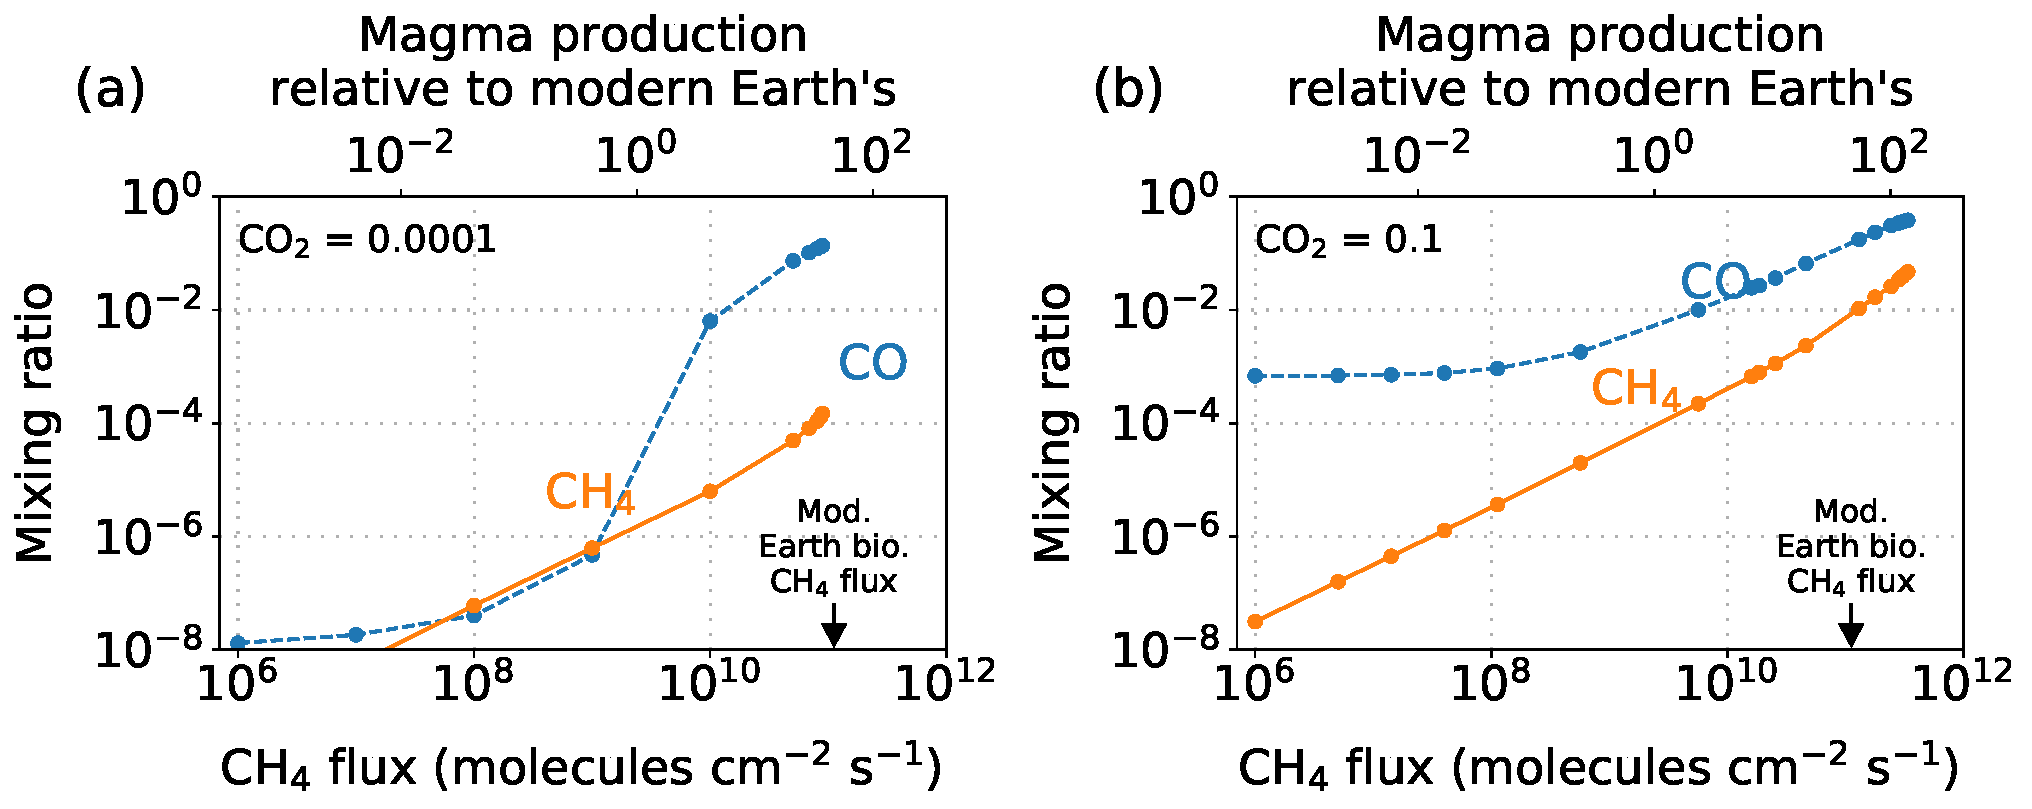
\includegraphics[width=\textwidth]{tex/3methane/figures/Figure5.pdf}
  \caption{Identical to Figure \ref{fig:photosun}, except for a planet that orbits a M8V star instead of a sun-like star.}
  \label{fig:photoM}
\end{figure*}

Figure \ref{fig:photoM} shows the CO and CH$_4$ mixing ratios on an Earth-sized ocean-world with reducing volcanic gases orbiting a cold M star. CO and CH$_4$ are more abundant on the ocean-world orbiting the M star compared to the ocean-world orbiting a Sun-like star (Figure \ref{fig:photosun}). This is because M8V stars have a low flux of near-ultraviolet radiation compared to sun-like stars. The low near-ultraviolet flux reduces OH produce from H$_2$O photolysis, thus allowing for relatively high CO and CH$_4$ concentrations. 

One consequence of M-dwarf photochemistry is a higher likelihood of Archean Earth-like CH$_4$ abundances on uninhabited planets with reducing gases from volcanism. Figure \ref{fig:photoM} shows that modern Earth magma production rates can result in CH$_4$ abundances up to 0.01\% which is comparable to what is expected in the Archean atmosphere. 

Potential CH$_4$ biosignature false positives from reducing volcanic gases might be discriminated from inhabited worlds using observations of CO. For planets orbiting Sun-like stars (Figure \ref{fig:photosun}) or M stars (Figure \ref{fig:photoM}) the CO abundance is higher than the CH$_4$ abundance in every case that is a potential outgassing false-positive. Some authors have argued that a large CO abundance is unlikely on an inhabited planet, because atmospheric CO should be readily consumed by biology \citep{Krissansen-Totton_2018a}. Conversely, \citet{Schwieterman_2019} has demonstrated hypothetical cases where large CO can coincide with with biology in an anoxic atmosphere. We further discuss CO as a false-positive discriminant in Section \ref{sec:CO_disc}.

\section{Discussion}

\subsection{The reasons why volcanoes produce little CH$_4$} \label{sec:littleCH4}

Our modeling results show that for modern Earth magma production rates, volcanic fluxes of reducing gases are unlikely to produce more than 1 Tmol CH$_4$/yr even in an extreme case (Figure \ref{fig:CH4}). This flux is relatively small compared to the flux of other volcanic gases on modern Earth. For example, Earth's modern volcanoes produce about ~7.5 Tmol CO$_2$/yr and ~95 Tmol H$_2$O/yr \citep[p. 203]{Catling_2017}. There are three main reasons why the outgassing model predicts little CH$_4$, which we discuss below.

\subsubsection{Volcanoes produce little CH$_4$ because of water solubility in magma} \label{sec:water_solu}

One reason for small CH$_4$ outgassing is the high solubility of water in magma at high pressures. Consider Equation \eqref{eq:react3}, which can be re-arranged to the following
\begin{equation}\label{eq:react3.1}
    \frac{P_{\mathrm{CH_4}}}{P_{\mathrm{CO_2}}}=\frac{K_3 P_\mathrm{H_2O}^2}{f_\mathrm{O_2}^2}
\end{equation}
The ratio $P_{\mathrm{CH_4}}/P_{\mathrm{CO_2}}$ in a gas bubble in magma is directly proportional to $P_\mathrm{H_2O}^2$ within that bubble. Generally speaking, $P_\mathrm{H_2O}$ increases as the total pressure of degassing increases because all partial pressures must sum to the total pressure (Equation \eqref{eq:pres}). For example, subaerial degassing at $\sim$1 bar will have a relatively small $P_\mathrm{H_2O}$, and thus a small $P_{\mathrm{CH_4}}/P_{\mathrm{CO_2}}$ ratio. On the other hand, submarine degassing at $\sim$400 bar should have a larger H$_2$O partial pressure, and thus a larger $P_{\mathrm{CH_4}}/P_{\mathrm{CO_2}}$ ratio. Here, the equilibrium constant and oxygen fugacity have extremely weak pressure dependencies, i.e. they are effectively constant as degassing pressure changes.

\begin{figure*}
  \centering
  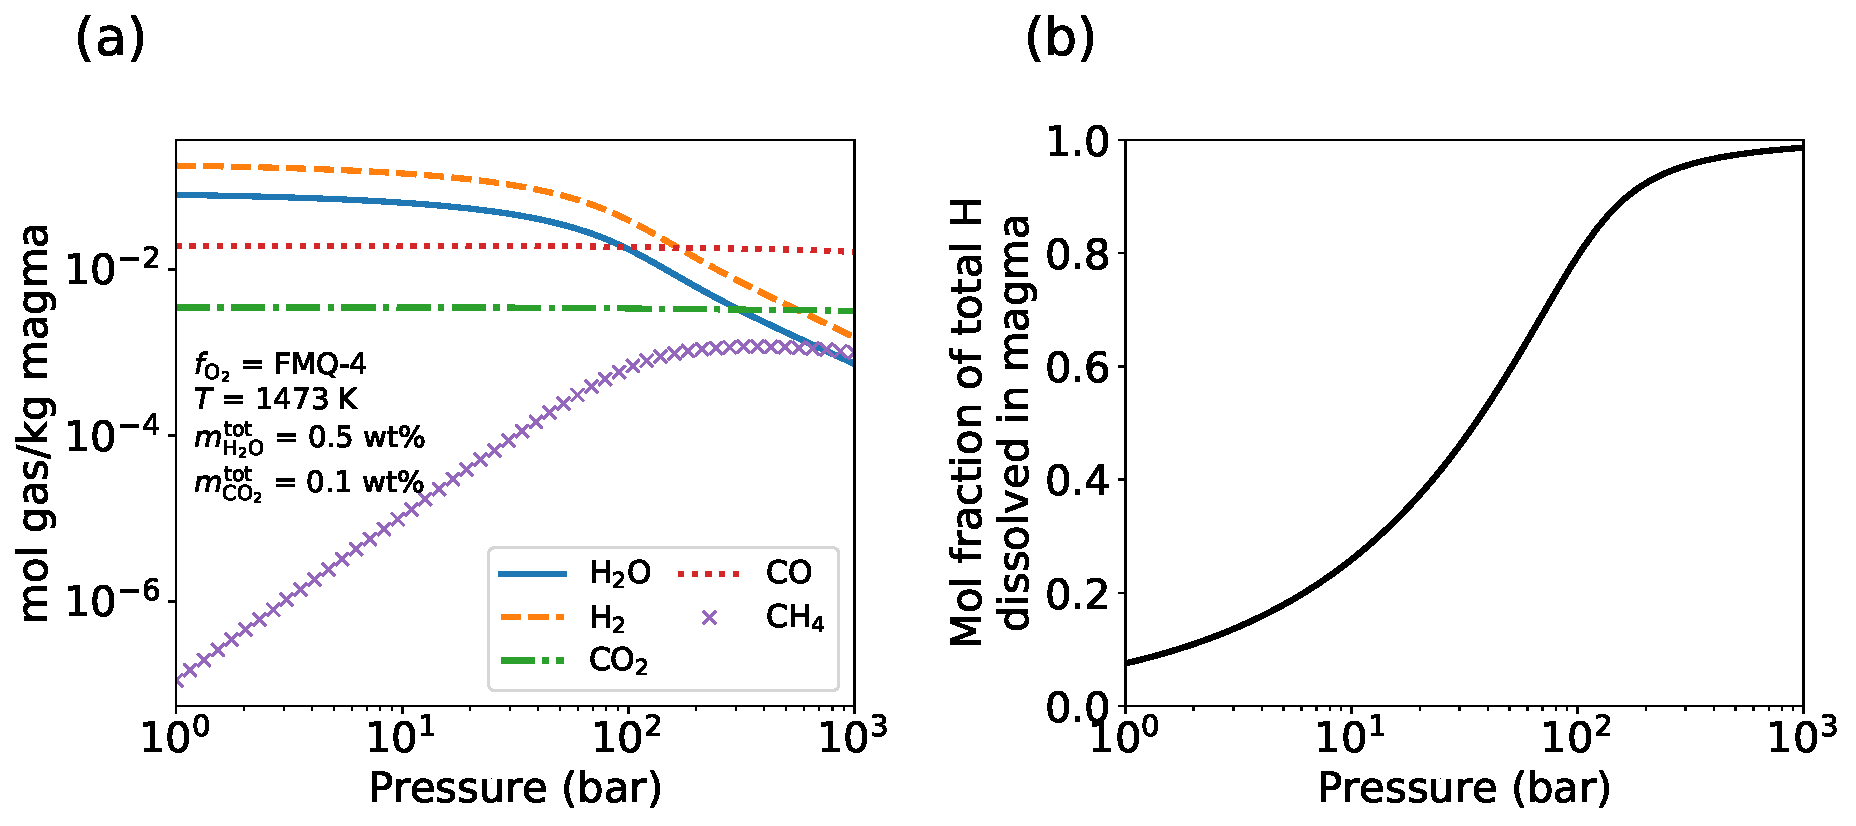
\includegraphics[width=\textwidth]{tex/3methane/figures/P_dependence.pdf}
  \caption{(a) Modeled gases speciation as a function of pressure. (b) Mole fraction of total hydrogen dissolved in the magma as a function of pressure. Model assumes $f_\mathrm{O_2}=$ FMQ-4, $T=1473$ K, $m_\mathrm{H_2O}^\mathrm{tot}$ = 0.5 wt\%, and $m_\mathrm{CO_2}^\mathrm{tot}$ = 0.1 wt\%. Methane becomes more prevalent in volcanic gases at higher pressures, but asymptotes because hydrogen dissolves into the magma, reducing the total amount of H-bearing volatiles released from the magma.}
  \label{fig:P_dependence}
\end{figure*}

Figure \ref{fig:P_dependence}a shows modeled gas speciation for highly reducing volcanism ($f_\mathrm{O_2}=$ FMQ-4) as a function of pressure. For small pressures ($<100$ bar), CH$_4$ increases with increasing pressure and then asymptotes for pressures $>100$ bar.

CH$_4$ asymptotes because of the high solubility of water in magma at high pressure. High pressures dissolve a large fraction of the total available hydrogen as H$_2$O into the magma, which is shown in Figure \ref{fig:P_dependence}b. Dissolving a large amount of H$_2$O into the magma limits the amount of hydrogen available in the gas phase for making H-bearing species, like CH$_4$, H$_2$O and H$_2$. 

In summary, high pressure is in some ways thermodynamically favorable for making methane because $P_{\mathrm{CH_4}}/P_{\mathrm{CO_2}} \propto P_\mathrm{H_2O}^2$, but also unfavorable because high pressure dissolves a large fraction of the available hydrogen in the magma as H$_2$O. Limited amounts of hydrogen in gas bubbles results in small amounts of CH$_4$ produced.

\citet{Kasting1998} used Equation \eqref{eq:react3.1} to argue that $\sim$1\% of the carbon outgassed by submarine volcanoes should be CH$_4$ for magma with $f_\mathrm{O_2} = \mathrm{FMQ}$. They assumed that $P_\mathrm{H_2O} \approx P$, the total pressure. This assumption is valid for oxidized subaerial volcanoes because $\sim$90\% of the gas exsolved by Earth's subaerial volcanoes is H$_2$O \citep[p. 203]{Catling_2017}. However, $P_\mathrm{H_2O} < P$ for submarine volcanoes because of the high-water solubility in magma at high pressure. Our outgassing model, which accounts for water's solubility in magma, produces negligible methane.

\citet{Li_2004} also predict abundant CH$_4$ produced by subaerial and submarine volcanoes (their Figure 5). However they calculated equilibrium constants in units of bars, but then used units of Pascals for equilibrium chemistry calculations. The result was that they calculated speciation for pressures a factor 10,000 times greater than reported. For example, we were able to reproduce their subaerial outgassing case (their Figure 5a) by assuming $P=10,000$ bar and not the $P=1$ bar total pressure they intended. Additionally, like \citet{Kasting1998}, they did not account for the high solubility of H$_2$O in magma at high pressure. Their methods assume the total hydrogen outgassed for submarine volcanoes is the same as the total hydrogen outgassed by subaerial volcanoes. This should not be the case because at high pressure water dissolves in magma and is unavailable for making H-bearing gas species (Figure \ref{fig:P_dependence}b).

The pressure dependence of volcanic outgassing has implications for planetary atmospheres generally \citep{Gaillard_2014}. Thin atmospheres will allow substantial degassing of both carbon and hydrogen bearing species. However, planets with thick atmospheres or large global oceans will have volcanic degassing dominated by CO$_2$ and CO, and almost no hydrogen bearing species. The overburden pressure where C-bearing species dominate depends primarily on the un-degassed concentrations of H$_2$O and CO$_2$ in the magma. In Figure \ref{fig:P_dependence}, CO$_2$ and CO overwhelms H-bearing species at $\sim$1000 bar for initial volatile concentrations of $m_\mathrm{CO_2}^\mathrm{tot} = 0.1$\%, and $m_\mathrm{H_2O}^\mathrm{tot} = 0.5$\%. In contrast, Figure 8 in \citet{Gaillard_2014} illustrates a case with less volatiles ($m_\mathrm{CO_2}^\mathrm{tot} = 0.007$\% and $m_\mathrm{H_2O}^\mathrm{tot} = 0.03$\%) where C-bearing species eclipse H-bearing species at $\sim$1 bar.

\subsubsection{Volcanoes produce little CH$_4$ because magma is hot}

Relatively little CH$_4$ is produced by volcanoes because CH$_4$ is generally not thermodynamically favorable at typical magma degassing temperatures. Figure \ref{fig:T_dep} shows gas speciation as a function of temperature for a submarine outgassing case. For these chosen inputs, CH$_4$ is the dominant carbon-bearing species for $T<1200$ K. Mid-ocean ridge basalts (MORB) are about 2/3 of total magma produced on Earth \citep{Crisp_1984}. MORB magma erupt at temperatures between 1473 K and 1650 K \citep{Scheidegger_1973} and are thus in a temperature regime where CH$_4$ is unfavorable even from more reducing volcanism.

\begin{figure}
    \centering
    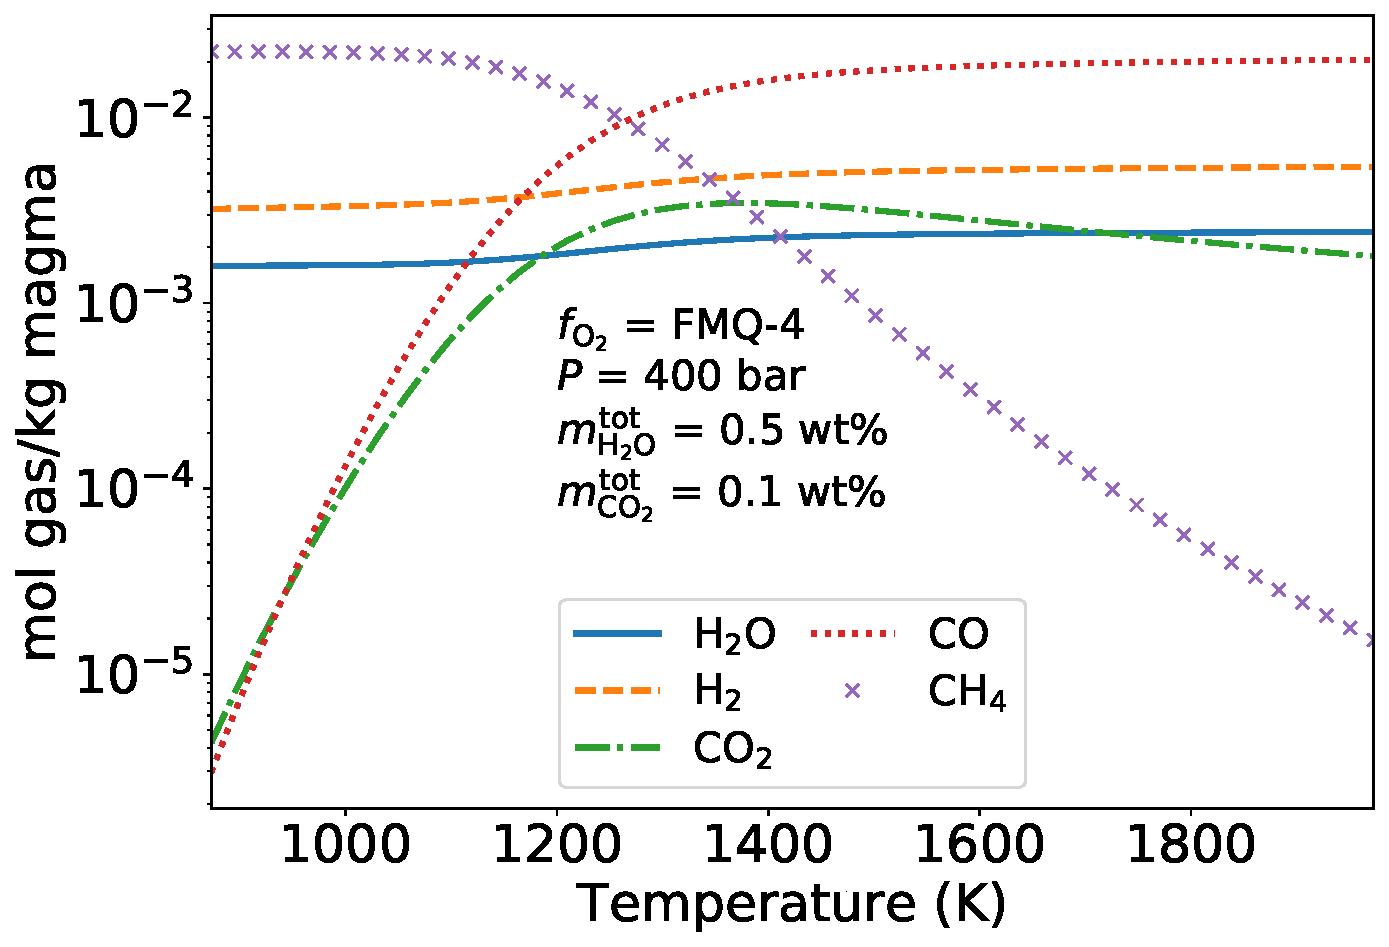
\includegraphics[width=10 cm]{tex/3methane/figures/T_dependence.pdf}
    \caption{Modeled volcanic outgassing speciation as a function of temperature. Model assumes $f_\mathrm{O_2}=$ FMQ-4, $P=400$ bar, $m_\mathrm{H_2O}^\mathrm{tot}$ = 0.5 wt\%, and $m_\mathrm{CO_2}^\mathrm{tot}$ = 0.1 wt\%. CH$_4$ is more thermodynamically favorable at lower degassing temperatures.}
    \label{fig:T_dep}
\end{figure}

On the other hand, magma from arc volcanoes is generally much colder than MORB magma. \citet{Moussallam_2019} report magma temperatures for many arc volcanoes (their Table S3), the coldest of which are 1123 K. Thus, it does seem possible for magma to be cold enough for CH$_4$ to be the dominant carbon-bearing outgassed species from an extremely reducing volcano with $f_\mathrm{O_2}=$ FMQ-4.

Recall that large magma production rates ($\sim$30x modern) are required for volcanoes to produce CH$_4$ fluxes compared to biological ones (Figure \ref{fig:photosun}). It seems unlikely that planets with large magma production rates will have magma temperatures cold enough to produce plentiful CH$_4$. For example, the Archean Earth may have had a larger magma production rate than the modern Earth because the Earth's mantle was hotter on the distant past \citep{Sleep_2001}. The hotter Archean mantle resulted in the eruption of $\sim$1800 K komatiite magmas \citep{Huppert_1984}, or possibly only $\sim$1600 K \citep{McKenzie_2020}. Such hot magma degassing is unfavorable for methane (Figure \ref{fig:T_dep}).

\subsubsection{Volcanoes produce little CH$_4$ because very low oxygen fugacity is required}

The final reason why volcanic CH$_4$ is unlikely on terrestrial planets is because very low $f_\mathrm{O_2}$ is required to make abundant methane. Figure \ref{fig:fO2} shows gas speciation as a function of oxygen fugacity for submarine volcanism. For these assumed inputs, methane is a substantial fraction of outgassed species for $f_\mathrm{O_2}<$ FMQ-3, and at FMQ-5 (roughly equivalent to the quartz-fayalite-iron buffer) half the carbon is converted to CH$_4$, while the other half is CO. Most degassing on Earth occurs at approximately $f_\mathrm{O_2}=\mathrm{FMQ}$ \citep[p. 208]{Catling_2017}, but magma spans FMQ-4 to FMQ+5 \citep{Stamper_2014}. Additionally, the oxygen fugacity of Martian meteorites ranges between FMQ and FMQ-3.7 \citep[p. 363]{Catling_2017}. Therefore, the $f_\mathrm{O_2}<$ FMQ-3 required for plentiful CH$_4$ outgassing is at the extremes of the oxygen fugacities observed for Earth and Mars. 

Astronomical observations and geochemical experiments suggest Earth-sized planets should generally have relatively oxidized magmas. \citet{Doyle_2019} spectroscopically measured the oxygen fugacity of material polluting the surface of several white dwarfs. Their observations suggest that rocky exoplanets are likely to have similar oxygen fugacities to Earth and Mars. Additionally, high pressure experiments suggest that the upper mantles of Earth-sized planets should self-oxidize by iron oxide disproportionation to roughly FMQ during the magma-ocean phase, early in a planet's life \citep{Armstrong_2019}.

\begin{figure}
    \centering
    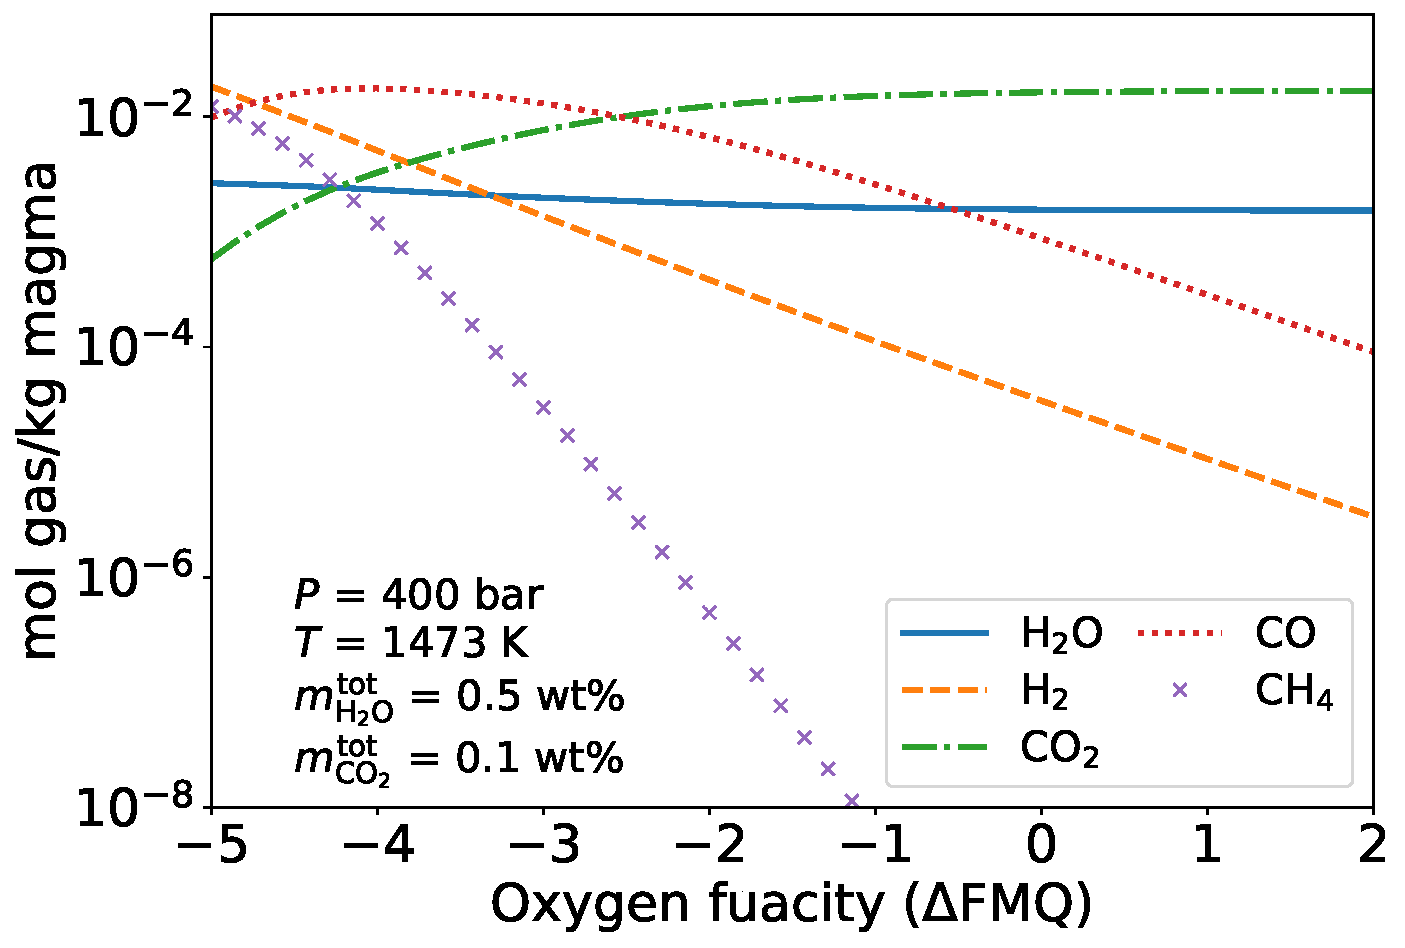
\includegraphics[width=10 cm]{tex/3methane/figures/fO2_dependence.pdf}
    \caption{Modeled volcanic outgassing speciation as a function of oxygen fugacity. Model assumes $P=400$ bar, $T=1473$ K, $m_\mathrm{H_2O}^\mathrm{tot}$ = 0.5 wt\%, and $m_\mathrm{CO_2}^\mathrm{tot}$ = 0.1 wt\%. Methane is most favorable at low oxygen fugacity.}
    \label{fig:fO2}
\end{figure}

\subsection{Carbon monoxide as a methane biosignature discriminant} \label{sec:CO_disc}

CO-consuming life evolved very early on Earth \citep{Adam_2018} and is a relatively simple metabolism. Therefore, it seems possible that life on other planets will evolve to consume CO. Planets with atmospheric CH$_4$+CO$_2$ produced by life might also have relatively small amounts of atmospheric CO because of CO consumers. Consequentially, the presence of abundant CO along with CH$_4$ can discriminate abiotic situations.

Monte-Carlo simulations shows that volcanoes should almost always produce more CO than CH$_4$ (Figure \ref{fig:result1}). Additionally, photochemical modeling (Figure \ref{fig:photosun} and \ref{fig:photoM}) suggests that CO should build up in the atmospheres of uninhabited planets with reducing submarine volcanic gases. Thus, atmospheric CO$_2$+CH$_4$ produced by volcanoes is likely accompanied by a large CO concentration. This is distinct from an inhabited world, which can have lower CO concentrations due to CO consuming life. 

However, the mere presence of large atmospheric CO is not a definitive sign of an uninhabited planet with reducing volcanic gases \citep{Schwieterman_2019}. This is because there are limits to how quickly gases can be transported from the atmosphere, into the ocean where they can be consumed by life \citep{Kharecha_2005}. For example, consider a planet with a very large volcanic CO flux (e.g., 100x modern). CO could build up in this planet's atmosphere even if CO consumers were present in an ocean because CO transport from the atmosphere to the ocean would not be sufficient to maintain low atmospheric CO. 

In summary, the CH$_4$+CO$_2$ biosignature is most compelling when the CO abundance is low or negligible because lack of CO potentially implies the presence of CO consuming biology. In comparison, atmospheric CH$_4$+CO$_2$ and large CO is ambiguous, and can either be explained by reducing volcanic gases or by an inhabited world that is unable to sequester atmospheric CO.

JWST might be able to put a tentative upper limit on atmospheric CO. \citet{Krissansen-Totton_2018a} simulated JWST retrievals of TRAPPIST-1e with an atmospheric composition similar to the Archean Earth containing 10 ppbv CO. Their synthetic retrieval suggested CO was below 652 ppmv with 90\% confidence after 10 transits. CO constraints could be improved by co-adding more transits and positive CO detections may also be possible with JWST \citep{Wunderlich_2020}.

However, even if observational CO constraints are poor, it may still be possible to say something about the abiotic or biotic origin of atmospheric CH$_4$. Reducing gases from volcanism are unlikely to mimic the modern biological CH$_4$ flux of 30 Tmol/yr (Section \ref{sec:littleCH4}). Additionally, serpentinization is unlikely to produce 30 Tmol CH$_4$/yr, and impact-generated CH$_4$ might be distinguished with system age \citep{Krissansen-Totton_2018b}. Therefore, JWST observations of atmospheric CH$_4$+CO$_2$ would be challenging to explain without the presence of biology regardless of atmospheric CO, as long as the CH$_4$ abundance implies a surface flux similar to the modern Earth's.

\subsection{CH$_4$ levels and implications for the origin on life}

Much current origin of life research revolves around the ``RNA world'' hypothesis \citep{Gilbert_1986,Joyce_2018,Sasselov_2020}. This hypothesis proposes an interval of time when primitive life consisted of self-replicating, evolving RNA molecules, which, at some point, were encapsulated in cells. On a rocky world, ``RNA world'' requires that RNA is synthesized from early raw materials. Laboratory experiments that have successfully synthesized nucleobases, which are building blocks of RNA, require the following nitriles: hydrogen cyanide (HCN), cyanoacetylene (HCCCN), and cyanogen (NCCN) \citep{Sutherland_2016,Ritson_2018,Benner_2019}. In addition, nitriles have also been used to synthesize amino acids \citep{Miller_1959,Sutherland_2016}.

The known natural source of nitriles is photochemistry in a chemically reducing atmosphere containing H$_2$, CH$_4$ and N$_2$ or perhaps NH$_3$. For example, Titan's photochemistry produces all the aforementioned nitriles \citep{Strobel_2009}. Importantly, to make the simplest nitrile, HCN, requires abundant CH$_4$ because HCN is formed from photochemical products of CH$_4$ and nitrogen \citep{Zahnle_1986,Tian_2011}.

Our results show that volcanic gases generally are unlikely to cause high atmospheric CH$_4$ abundances in prebiotic atmospheres. Consequently, the results lend credence to alternative proposals for making early CH$_4$-rich, reducing atmospheres, such as impacts \citep{Zahnle_2020}. Impacts can make a reducing atmosphere when reactions between iron-rich impact ejecta and shock-heated water vapor from an ocean generate copious H$_2$, CH$_4$ and NH$_3$. Subsequent photochemistry would generate HCN and other prebiotic nitriles over thousands to millions of years \citep{Zahnle_2020}.

\section{Conclusions}

Our modeling of volcanic outgassing speciation suggests that chemically reducing volcanism on terrestrial planets is unlikely to mimic biological CH$_4$ fluxes. The improbable cases where volcanoes do produce biological CH$_4$ fluxes also often produce CO. Volcanoes are not prone to produce CH$_4$ for several reasons. First, the high solubility of H$_2$O in magma limits the amount of total hydrogen outgassed, thus preventing the production of H-bearing molecules like CH$_4$. Second, CH$_4$ outgassing requires relatively low magma temperatures compared to the majority of magma erupted on Earth. Finally, CH$_4$ outgassing requires a very low magma oxygen fugacity unlike that of most terrestrial planets inferred from astronomical data \citep{Doyle_2019}.

We use a photochemical model to calculate atmospheric composition of planets with volcanoes that produce CH$_4$. We find that atmospheric CH$_4$ should coincide with abundant CO. On the other hand, biogenic CH$_4$ can coincide with a low CO abundance if CO-consuming microbial life is present.

Therefore, the CH$_4$-CO$_2$ biosignature is most compelling when little or no atmospheric CO is detected. Atmospheric CH$_4$-CO$_2$ and large CO is ambiguous and can be explained by an uninhabited planet with highly reducing volcanic gases, or an inhabited planet where biology is unable to sequester atmospheric CO \citep{Schwieterman_2019}.

However, observations of CO are not required to make conclusions about the abiotic or biotic origin of observed atmospheric CH$_4$. Atmospheric CH$_4$ and CO$_2$ alone would have a reasonable probability of being biological if the observed CH$_4$ abundance implies a surface flux similar to modern Earth’s biological CH$_4$ flux (30 Tmol/yr). Such a large CH$_4$ flux is difficult to explain with reducing volcanic gases or other abiotic processes that generate CH$_4$, such as serpentenization.

These conclusions should be taken with caution because they are based on what is understood about processes occurring on the Earth and our Solar System, which may be a very sparse sampling of what is possible.

\section{Chapter Appendix}

\subsection{Details of outgassing speciation model}

\subsubsection{Solubility constants for of H$_2$O and CO$_2$} \label{sec:solu_constants}
Our outgassing model uses solubility equations for H$_2$O and CO$_2$ in mafic magmas from \citet{Iacono-Marziano_2012} (Equations \eqref{eq:solu1} and \eqref{eq:solu2}). The parameters $S_1$ and $S_2$ in the solubility equations depend on the chemical make-up of the magma. We found that different mafic magma compositions did not significantly effect the outputs of our outgassing speciation model (Section \ref{sec:volcmodel}), therefore, for the purposes of calculating melt solubility, we fixed the chemical make-up of the magma to the magma erupting at Mt. Etna, Italy, reported by \citet{Iacono-Marziano_2012}. This reduced the complexity of the model without sacrificing any significant amount of accuracy.

Table \ref{tab:magmacomp} shows the chemical make-up of the magma at Mt. Etna, and Table \ref{tab:soluconst} shows several solubility constants from \citet{Iacono-Marziano_2012}. Together these values define the solubility parameters $S_1$ and $S_1$:
\begin{equation}
\begin{split}
    {S_1} &= \ln \left(\frac{\mu_\mathrm{magma}}{\mu_\mathrm{CO_2}10^{6}}\right) + \frac{{{C_{{\text{C}}{{\text{O}}_{\text{2}}}}}P}}{T} + {B_{{\text{C}}{{\text{O}}_{\text{2}}}}} + {b_{{\text{C}}{{\text{O}}_{\text{2}}}}}\left[ {\frac{{{\text{NBO}}}}{{\text{O}}}} \right] \\
    &+ \left( {\frac{{{x_{{\text{A}}{{\text{l}}_{\text{2}}}{{\text{O}}_{\text{3}}}}}}}{{{x_{{\text{CaO}}}} + {x_{{{\text{K}}_{\text{2}}}{\text{O}}}} + {x_{{\text{N}}{{\text{a}}_{\text{2}}}{\text{O}}}}}}} \right){d_{{\text{A}}{{\text{l}}_{\text{2}}}{{\text{O}}_{\text{3}}}{\text{/(CaO + }}{{\text{K}}_{\text{2}}}{\text{O + N}}{{\text{a}}_{\text{2}}}{\text{O)}}}}\\
    &+ ({x_{{\text{FeO}}}} + {x_{{\text{MgO}}}}){d_{{\text{FeO + MgO}}}} + ({x_{{\text{N}}{{\text{a}}_{\text{2}}}{\text{O}}}} + {x_{{{\text{K}}_{\text{2}}}{\text{O}}}}){d_{{\text{N}}{{\text{a}}_2}{\text{O + }}{{\text{K}}_2}{\text{O}}}}
\end{split}
\end{equation}
\begin{equation}
    {S_2} = \ln \left(\frac{\mu_\mathrm{magma}}{{\mu_{{{\text{H}}_2}{\text{O}}}}10^2}\right) + \frac{{{C_{{{\text{H}}_2}{\text{O}}}}P}}{T} + {B_{{{\text{H}}_2}{\text{O}}}} + {b_{{{\text{H}}_2}{\text{O}}}}\left[ {\frac{{{\text{NBO}}}}{{\text{O}}}} \right]
\end{equation}
\begin{equation}
    \left[ {\frac{{{\text{NBO}}}}{{\text{O}}}} \right] = \frac{{2({x_{{{\text{K}}_{\text{2}}}{\text{O}}}} + {x_{{\text{N}}{{\text{a}}_{\text{2}}}{\text{O}}}} + {x_{{\text{CaO}}}} + {x_{{\text{MgO}}}} + {x_{{\text{FeO}}}} - {x_{{\text{A}}{{\text{l}}_{\text{2}}}{{\text{O}}_{\text{3}}}}})}}{{2{x_{{\text{Si}}{{\text{O}}_{\text{2}}}}} + 2{x_{{\text{Ti}}{{\text{O}}_{\text{2}}}}} + 3{x_{{\text{A}}{{\text{l}}_{\text{2}}}{{\text{O}}_{\text{3}}}}} + {x_{{\text{MgO}}}} + {x_{{\text{FeO}}}} + {x_{{\text{CaO}}}} + {x_{{\text{N}}{{\text{a}}_{\text{2}}}{\text{O}}}} + {x_{{{\text{K}}_{\text{2}}}{\text{O}}}}}}
\end{equation}
Here, $T$ is magma temperature, $P$ is the total pressure of degassing, and $\left[\frac{\mathrm{NBO}}{\mathrm{O}}\right]$ is the amount of non-bridging oxygen per oxygen in the melt.

\begin{table}[]
  \caption{Mt. Etna magma composition}
  \label{tab:magmacomp}
  \centering
  \begin{tabular}{l c}
  \hline \hline
  Magma component & Mole fraction \\
  \hline
  $x_\mathrm{SiO_2}$     & 0.516   \\
  $x_\mathrm{TiO_2}$     & 0.014   \\
  $x_\mathrm{Al_2O_3}$     & 0.110   \\
  $x_\mathrm{FeO}$     & 0.091   \\
  $x_\mathrm{MgO}$     & 0.092   \\
  $x_\mathrm{CaO}$     & 0.126   \\
  $x_\mathrm{Na2O}$     & 0.035   \\
  $x_\mathrm{K_2O}$     & 0.002   \\
  $x_\mathrm{P_2O_5}$     & 0.016   \\
  \hline
  \multicolumn{2}{l}{Note. Taken from \citet{Iacono-Marziano_2012}.} 
  \end{tabular}
\end{table}

\begin{table}
  \caption{Solubility constants}
  \label{tab:soluconst}
  \centering
  \begin{tabular}{l c}
  \hline \hline
  Constant & Value \\
  \hline
  $C_\mathrm{CO_2}$     & 0.14   \\
  $B_\mathrm{CO_2}$     & -5.3   \\
  $b_\mathrm{CO_2}$     & 15.8   \\
  $B_\mathrm{H_2O}$     & -2.95   \\
  $b_\mathrm{H_2O}$     & 1.24   \\
  $d_\mathrm{Al_2O_3/(CaO+K_2O+Na_2O)}$     & 3.8   \\
  $d_\mathrm{FeO+MgO}$     & -16.3   \\
  $d_\mathrm{Na_2O+K_2O}$     & 20.1   \\
  \hline
  \multicolumn{2}{l}{Note. ``Anhydrous'' case from \citet{Iacono-Marziano_2012}.} 
  \end{tabular}
\end{table}

\subsubsection{Derivation of Equations \eqref{eq:C_con} and \eqref{eq:H_con}} \label{sec:Derivation_con}

Following is the derivation for the atom conservation equation for carbon used in our outgassing model (Equation \eqref{eq:C_con}). The derivation for the atom conservation equation for hydrogen follows the exact same procedure, so we do not include it. 

Consider some volume of magma with gas bubbles in it which contains a total number of moles $\gamma_\mathrm{tot}$. The total moles is the sum of the moles of magma ($\gamma_\mathrm{magma}$), and the moles of gas in bubbles suspended in that magma ($\gamma_\mathrm{gas}$):
\begin{equation} \label{eq:tot_con}
    \gamma_\mathrm{tot} = \gamma_\mathrm{gas} + \gamma_\mathrm{magma}
\end{equation}
Within this same volume of magma, the total moles of carbon ($\gamma_\mathrm{C}^\mathrm{tot}$) is equal to the moles of carbon in the gas phase ($\gamma_\mathrm{C}^\mathrm{gas}$) and the moles of carbon dissolved in the magma ($\gamma_\mathrm{C}^\mathrm{magma}$) combined. 
\begin{equation} \label{eq:CO2_con}
    \gamma_\mathrm{C}^\mathrm{tot} = \gamma_\mathrm{C}^\mathrm{gas} + \gamma_\mathrm{C}^\mathrm{magma}
\end{equation}
We assume that the only carbon bearing molecule that can dissolve in the magma is CO$_2$, therefore $\gamma_\mathrm{C}^\mathrm{magma}=\gamma_\mathrm{CO_2}^\mathrm{magma}$. Dividing by $\gamma_\mathrm{tot}$ and expanding gives
\begin{equation} 
    \frac{\gamma_\mathrm{C}^\mathrm{tot}}{\gamma_\mathrm{tot}} = \frac{\gamma_\mathrm{gas}}{\gamma_\mathrm{tot}}\frac{\gamma_\mathrm{C}^\mathrm{gas}}{\gamma_\mathrm{gas}} + \frac{\gamma_\mathrm{magma}}{\gamma_\mathrm{tot}}\frac{\gamma_\mathrm{CO_2}^\mathrm{magma}}{\gamma_\mathrm{magma}}
\end{equation}
We can replace $\frac{\gamma_\mathrm{magma}}{\gamma_\mathrm{tot}}$ with $1-\frac{\gamma_\mathrm{gas}}{\gamma_\mathrm{tot}}$ using Equation \eqref{eq:tot_con}. This leaves us with
\begin{equation} 
    \frac{\gamma_\mathrm{C}^\mathrm{tot}}{\gamma_\mathrm{tot}} = \frac{\gamma_\mathrm{gas}}{\gamma_\mathrm{tot}}\frac{\gamma_\mathrm{C}^\mathrm{gas}}{\gamma_\mathrm{gas}} + \left(1-\frac{\gamma_\mathrm{gas}}{\gamma_\mathrm{tot}}\right)\frac{\gamma_\mathrm{CO_2}^\mathrm{magma}}{\gamma_\mathrm{magma}}
\end{equation}
Here, $\frac{\gamma_\mathrm{CO_2}^\mathrm{magma}}{\gamma_\mathrm{magma}}$ is just $x_\mathrm{CO_2}$ (the mol fraction of CO$_2$ in the magma, see Table \ref{tab:1}). Also, we assume that CO$_2$, CO and CH$_4$ are the only carbon-bearing gas species, so $\gamma_\mathrm{C}^\mathrm{gas}=\gamma_\mathrm{CO_2}^\mathrm{gas}+\gamma_\mathrm{CO}^\mathrm{gas}+\gamma_\mathrm{CH_4}^\mathrm{gas}$. Making substitutions gives
\begin{equation} 
    \frac{\gamma_\mathrm{C}^\mathrm{tot}}{\gamma_\mathrm{tot}} = \frac{\gamma_\mathrm{gas}}{\gamma_\mathrm{tot}}\frac{\gamma_\mathrm{CO_2}^\mathrm{gas}+\gamma_\mathrm{CO}^\mathrm{gas}+\gamma_\mathrm{CH_4}^\mathrm{gas}}{\gamma_\mathrm{gas}} + \left(1-\frac{\gamma_\mathrm{gas}}{\gamma_\mathrm{tot}}\right)x_\mathrm{CO_2}
\end{equation}
Assuming the ideal gas law, $\gamma_i^\mathrm{gas}/\gamma_\mathrm{gas}=P_i/P$. Also, to make the equation more manageable, we substitute $\alpha_\mathrm{gas}=\frac{\gamma_\mathrm{gas}}{\gamma_\mathrm{tot}}$, which is the total mols in the gas phase divided by the moles in the gas phase and magma combined.
\begin{equation} \label{eq:IDK}
    \frac{\gamma_\mathrm{C}^\mathrm{tot}}{\gamma_\mathrm{tot}} = \frac{P_\mathrm{CO_2}+P_\mathrm{CO}+P_\mathrm{CH_4}}{P}\alpha_\mathrm{gas} + \left(1-\alpha_\mathrm{gas}\right)x_\mathrm{CO_2}
\end{equation}
Magma sometimes freezes deep in the Earth as a glass before it releases any volatiles. Measurements of volatiles like CO$_2$, in such glasses are reported in terms of mass fractions \citep{Wallace_2015}. To stay consistent with these unit conventions, we indicate the total carbon in undegassed magma as a mass fraction of CO$_2$ ($m_\mathrm{CO2}^\mathrm{tot}$). We can convert the mass fraction to a mole fraction using Equation \eqref{eq:convert}:
\begin{equation} \label{eq:IDK2}
    \frac{m_\mathrm{CO2}^\mathrm{tot}\mu_\mathrm{magma}}{\mu_\mathrm{CO_2}}=x_\mathrm{CO2}^\mathrm{tot}=\frac{\gamma_\mathrm{CO_2}^\mathrm{tot}}{\gamma_\mathrm{tot}}=\frac{\gamma_\mathrm{C}^\mathrm{tot}}{\gamma_\mathrm{tot}}
\end{equation}
Substituting Equation \eqref{eq:IDK2} into Equation \eqref{eq:IDK} gives 
\begin{equation} \label{eq:LAST}
    {\frac{{m_{{\text{C}}{{\text{O}}_{\text{2}}}}^{{\text{tot}}}}\mu_\mathrm{magma}}{{{\mu_{{\text{C}}{{\text{O}}_{\text{2}}}}}}}} = \frac{{{P_{{\text{C}}{{\text{O}}_{\text{2}}}}} + {P_{{\text{CO}}}} + {P_{{\text{C}}{{\text{H}}_{\text{4}}}}}}}{P}{\alpha _{{\text{gas}}}} + (1 - {\alpha _{{\text{gas}}}}){x_{{\text{C}}{{\text{O}}_{\text{2}}}}}
\end{equation}
Equation \eqref{eq:LAST} is identical to Equation \eqref{eq:C_con}.

\subsubsection{Graphite saturation and the solubility of CO, CH$_4$, and H$_2$} \label{sec:graphite_sat}

Several studies have shown that degassing can be affected by graphite saturation of of magma \citep{Hirschmann_2008} or by the solubility of CO, CH$_4$, and H$_2$ in magma \citep{Wetzel_2013,Ardia_2013,Hirschmann_2012}. Our model for outgassing speciation used throughout the main text does not account for these complications. Here, we show that our assumption is valid because it does not significantly change our results.

Consider the following equilibrium.
\begin{equation}
    \mathrm{C}+\mathrm{O_2}\leftrightarrow\mathrm{CO_2}
\end{equation}
\begin{equation} \label{eq:graphite_sat}
    K_9=\frac{f_\mathrm{CO_2}}{a_\mathrm{C}f_\mathrm{O_2}}\approx \frac{P_\mathrm{CO_2}}{a_\mathrm{C}f_\mathrm{O_2}}
\end{equation}
Here, $K_9$ is the equilibrium constant given by $\exp(47457/T+0.136)$, and $a_\mathrm{C}$ is the activity of carbon. To incorporate graphite saturation into our model, we first calculate outgassing speciation using the model described in the main text (Section \ref{sec:volcmodel}). Next, we check for graphite saturate by calculating the activity of carbon using Equation \eqref{eq:graphite_sat}. If $a_\mathrm{C}<1$, then we assume the melt is not graphite saturated and that the calculation is valid. If $a_\mathrm{C}>1$, then we assume graphite is saturated and recalculate outgassing speciation by replacing the carbon conservation equation (Equation \eqref{eq:C_con}), with the graphite saturation equation  with $a_\mathrm{C}=1$ (Equations \eqref{eq:graphite_sat}). Here, we are considering graphite saturation in the magma just before degassing occurs. Our treatment is different than, for example, the methods of \citet{Ortenzi_2020} because they are accounting for graphite saturation much deeper in a planet during partial melting of the mantle.

Figure \ref{fig:graphite} is identical to Figure \ref{fig:result1}, except Figure \ref{fig:graphite} accounts for graphite saturation. Graphite saturation appears to have a small effect on the results, therefore it is justified to ignore it.

\begin{figure}
    \centering
    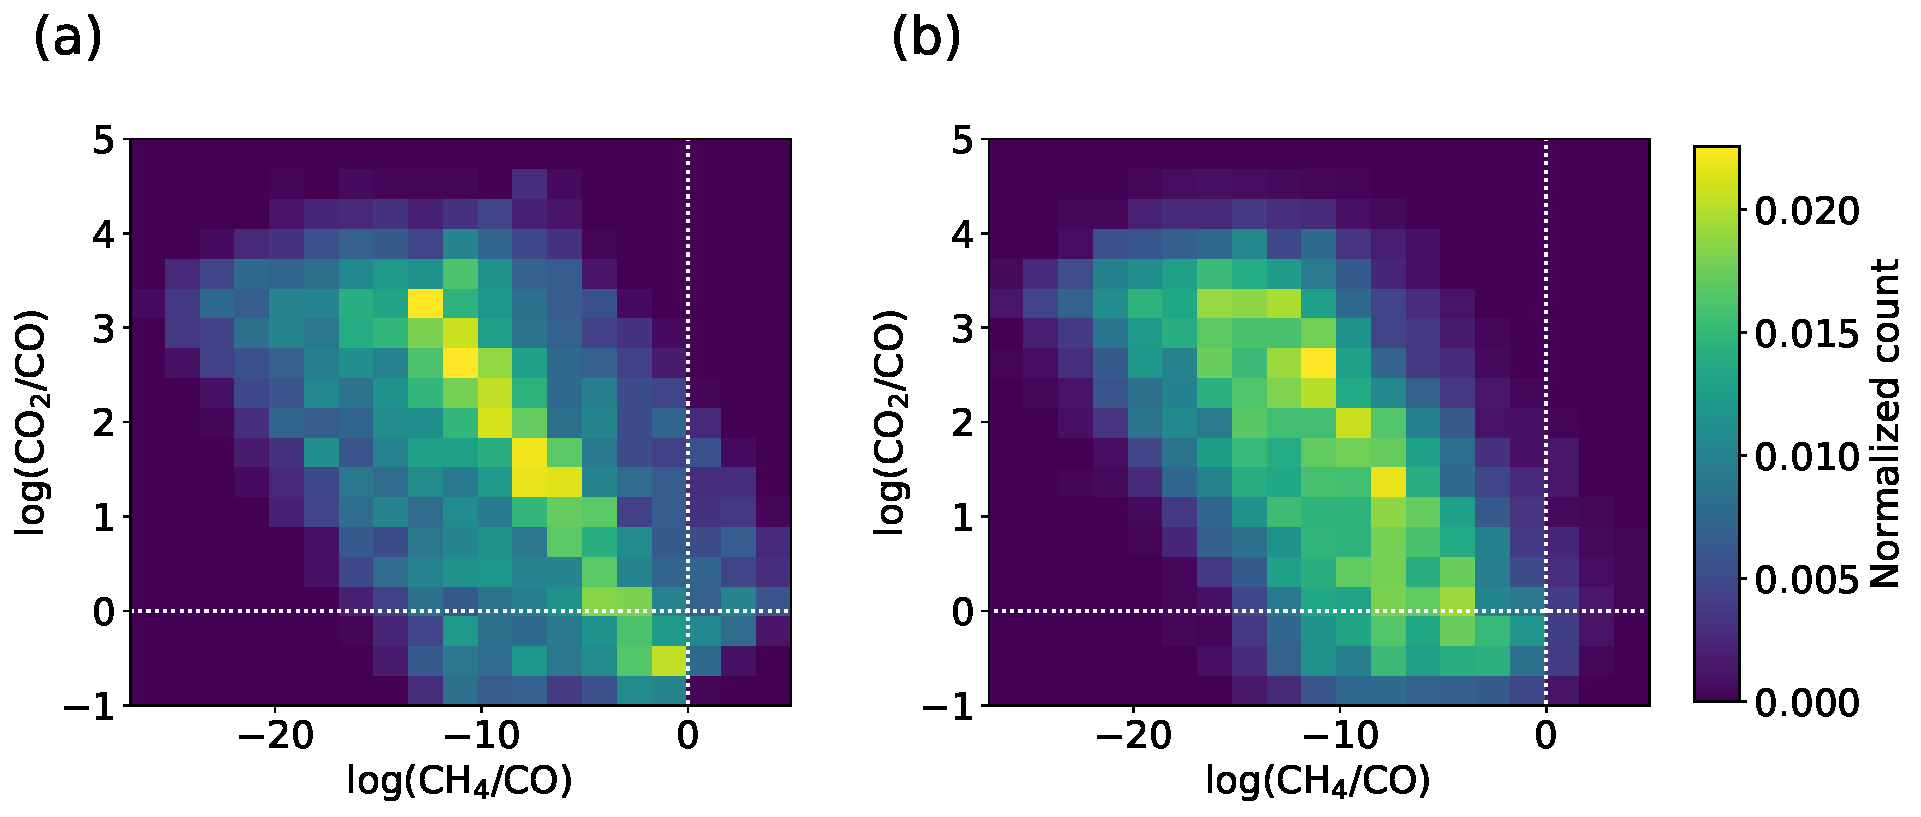
\includegraphics[width=\textwidth]{tex/3methane/figures/both_Csat.pdf}
    \caption{Identical to Figure \ref{fig:result1}, except here we account for graphite saturation in the melt. Like Figure \ref{fig:result1} (a) is for ocean worlds and (b) is for Earth-like worlds. Graphite saturation has a small effect on the results.}
    \label{fig:graphite}
\end{figure}

To incorporate the solubility of H$_2$, CH$_4$, and CO into our model, we add the following solubility relationships to or system of original outgassing equations (Section \ref{sec:volcmodel}).
\begin{equation}
    \exp(-11.403-0.000076P)=K_5=\frac{x_\mathrm{H_2}}{f_\mathrm{H_2}} \approx \frac{x_\mathrm{H_2}}{P_\mathrm{H_2}}
\end{equation}
\begin{equation}
    \exp(-7.63-0.000193P)=K_6=\frac{x_\mathrm{CH_4}}{f_\mathrm{CH_4}} \approx \frac{x_\mathrm{CH_4}}{P_\mathrm{CH_4}}
\end{equation}
\begin{equation} \label{eq:COsolub}
    \exp(-41.02-0.00056P) = K_7 = \frac{x_\mathrm{Fe(CO)_5}}{a_\mathrm{Fe}f_\mathrm{CO}^5} \approx \frac{x_\mathrm{Fe(CO)_5}}{a_\mathrm{Fe}P_\mathrm{CO}^5}
\end{equation}
Here, pressure dependent equilibrium constants $K_5$, $K_6$ and $K_7$ are from \citet{Hirschmann_2012}, \citet{Ardia_2013}, and \citet{Wetzel_2013}, respectively. For Equation \eqref{eq:COsolub}, we take the activity of iron to be $a_\mathrm{Fe}=0.6$ based on the experiments in \citet{Wetzel_2013}. Also, we only include the Equation \eqref{eq:COsolub} when the $f_\mathrm{O_2}<$ IW-0.55 (IW is the Iron-Wustite mineral buffer) because \citet{Wetzel_2013} only observed CO dissolved in magma for these low oxygen fugacities.

We also alter the carbon and hydrogen atom conservation equations to accommodate for new molecules in the melt.
\begin{equation} 
    \frac{m_\mathrm{CO_2}^\mathrm{tot}\mu_\mathrm{magma}}{\mu_\mathrm{CO_2}} = \frac{P_\mathrm{CO_2}+P_\mathrm{CO}+P_\mathrm{CH_4}}{P}\alpha_\mathrm{gas} + \left(1-\alpha_\mathrm{gas}\right)(x_\mathrm{CO_2}+x_\mathrm{CO}+x_\mathrm{CH_4})
\end{equation}
\begin{equation} 
    \frac{m_\mathrm{H_2O}^\mathrm{tot}\mu_\mathrm{magma}}{\mu_\mathrm{H_2O}} = \frac{P_\mathrm{H_2O}+P_\mathrm{H_2}+2P_\mathrm{CH_4}}{P}\alpha_\mathrm{gas} + \left(1-\alpha_\mathrm{gas}\right)(x_\mathrm{H_2O}+x_\mathrm{H_2}+2x_\mathrm{CH_4})
\end{equation}
Here, $x_i$ is the mol fraction of species $i$ in the melt.

Figure \ref{fig:Ch4COH2solu} is identical to Figure \ref{fig:result1}, except Figure \ref{fig:Ch4COH2solu} accounts for H$_2$, CH$_4$ and CO solubility in magma. The solubility of these three molecules has a small effect on the results, therefore they can be ignored.

\begin{figure}
    \centering
    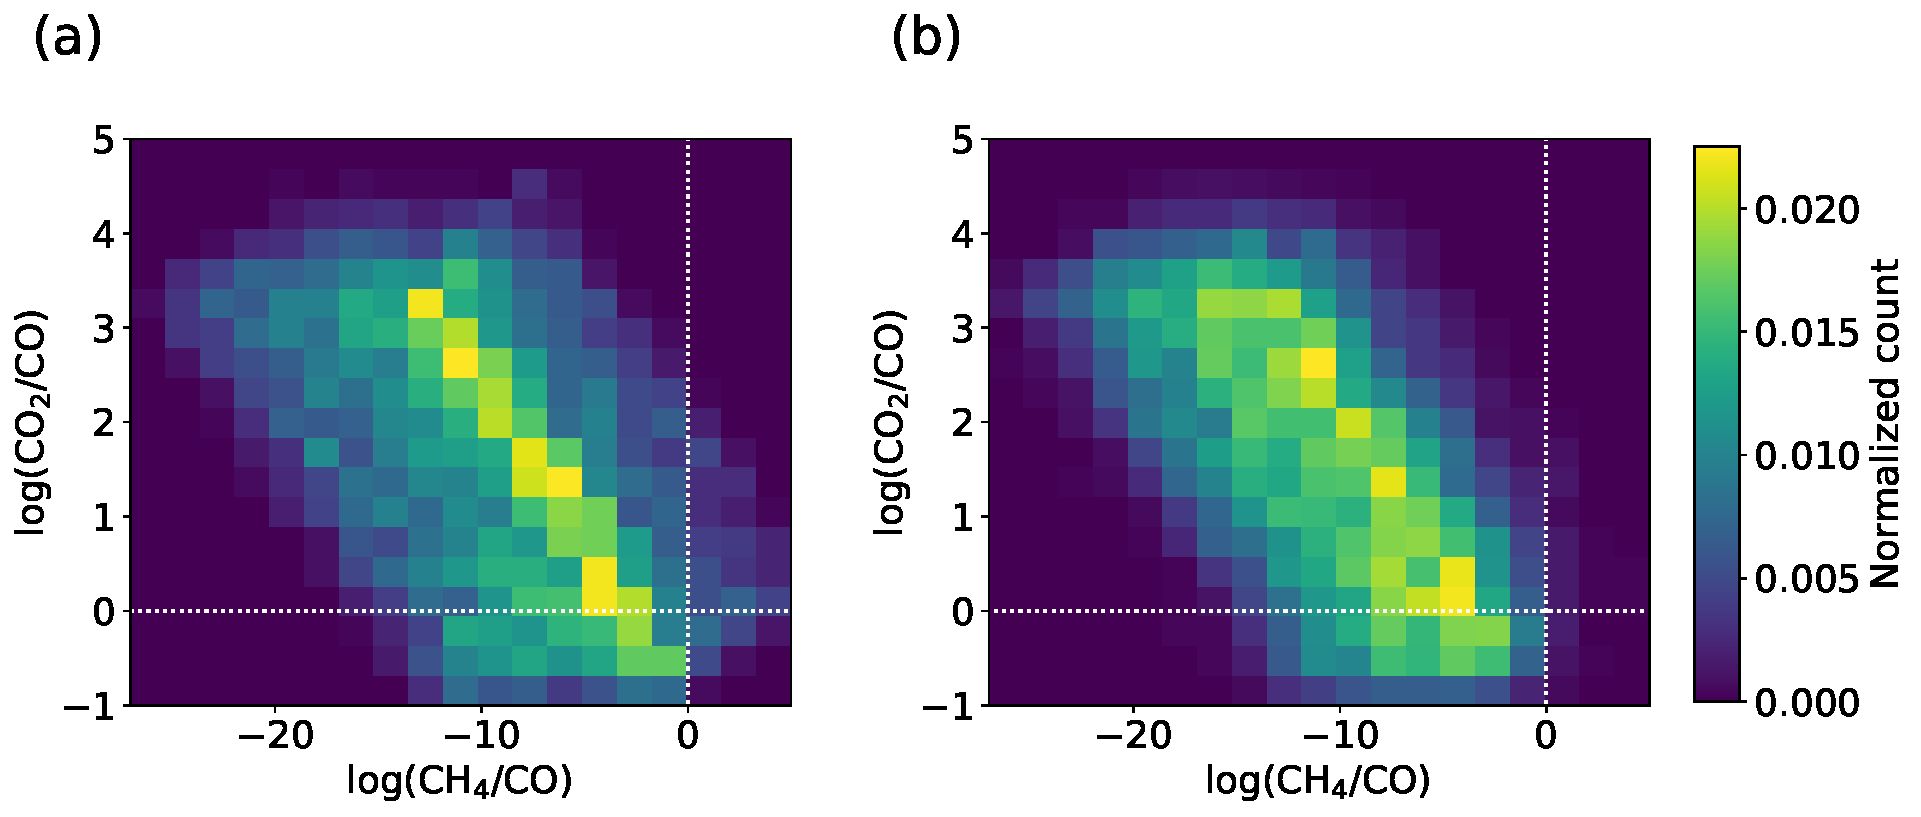
\includegraphics[width=\textwidth]{tex/3methane/figures/both_CO_H2_CH4_solu.pdf}
    \caption{Identical to Figure \ref{fig:result1}, except here we account for the solubility of H$_2$, CH$_4$ and CO in the melt. Like Figure \ref{fig:result1} (a) is for ocean worlds and (b) is for Earth-like worlds. H$_2$, CH$_4$ and CO  solubility has a small effect on the results.}
    \label{fig:Ch4COH2solu}
\end{figure}

\subsubsection{Closed system cooling and chemical kinetics}\label{sec:kinetics}

Our model for volcanic outgassing is a thermodynamic equilibrium model. We assume that during magma eruptions gas bubbles chemically and thermally equilibrate with magma, and then are released to the atmosphere unaltered (Figure \ref{fig:imagine}). This does not exactly reflect real degassing. 

In reality, the chemical composition of gas bubbles changes as bubbles leave the magma and enter the atmosphere \citep{Moussallam_2019, Kadoya_2020}. As a bubble leaves magma, it cools down, and new chemical equilibria are preferred. When the gas bubble first begins cooling, it is still very hot, so chemical reactions keep the bubble near chemical equilibrium. Once the bubble is cold enough, chemical reactions slow, and ultimately cease, quenching or freezing the chemical composition of the gas bubble. Therefore, the cooling process alters the chemistry of the gas. 

Gas re-equilibration to lower temperatures explains the observed chemistry of volcanic gases globally \citep{Moussallam_2019}, and \citet{Oppenheimer_2018} provides a specific example of this phenomenon at Kilauea volcano, Hawaii. During eruptions at Kilauea, gas bubbles in the magma would rise to the surface. As the bubbles rose in the magma, they adiabatically expanded, which cooled the gas below the temperature of the magma. Chemical reactions during adiabatic expansion changed the chemical make-up of the bubble.

For the purposes of understanding potential CH$_4$ biosignature false positives from volcanoes, we need to know if bubble cooling might generate a substantial amount of CH$_4$. Here, we first consider the kinetics of methane generation and show that reactions are likely too slow to generate substantial CH$_4$ during gas cooling. Next, we show that our Monte Carlo simulation results (Figure \ref{fig:CH4}) remain qualitatively unchanged even if our kinetics calculations are wrong, and CH$_4$ can be generated during gas cooling.

CO or CO$_2$ is converted to CH$_4$ through either of the net reactions \citep{Schaefer_2010}
\begin{equation}
    \mathrm{CO}+3\mathrm{H_2} \leftrightarrow \mathrm{CH_4} + \mathrm{H_2O}
\end{equation}
\begin{equation}
    \mathrm{CO_2}+4\mathrm{H_2} \leftrightarrow \mathrm{CH_4} + \mathrm{2H_2O}
\end{equation}
The rate limiting step to either CO or CO$_2$ conversion to CH$_4$ is debated in the literature \citep{Zahnle_2014}, but following are two good candidates and their corresponding rate constants:
\begin{equation}
    \mathrm{H_2}+\mathrm{H_2CO} \rightarrow \mathrm{CH_3} + \mathrm{OH}
\end{equation}
\begin{equation}
    k_{10} = 2.3\times10^{-10}\exp(-36200/T)
\end{equation}
\begin{equation}
    \mathrm{H}+\mathrm{H_2CO} \rightarrow \mathrm{CH_3} 
\end{equation}
\begin{equation}
    k_{12} = 4.0\times10^{-11}\exp(-2068/T)
\end{equation}
Here, $k_{10}$ and $k_{12}$ are rate constants (cm$^3$ s$^{-1}$). The lifetime of CO or CO$_2$ conversion to CH$_4$ is thus one of the following
\begin{equation} \label{eq:first_time}
    \tau_{10}(\mathrm{CO})=\frac{N_\mathrm{CO}}{k_{10}N_\mathrm{H_2}N_\mathrm{H_2CO}}
\end{equation}
\begin{equation}
    \tau_{12}(\mathrm{CO})=\frac{N_\mathrm{CO}}{k_{12}N_\mathrm{H}N_\mathrm{H_2CO}}
\end{equation}
\begin{equation}
    \tau_{10}(\mathrm{CO_2})=\frac{N_\mathrm{CO_2}}{k_{10}N_\mathrm{H_2}N_\mathrm{H_2CO}}
\end{equation}
\begin{equation} \label{eq:last_time}
    \tau_{12}(\mathrm{CO_2})=\frac{N_\mathrm{CO_2}}{k_{12}N_\mathrm{H}N_\mathrm{H_2CO}}
\end{equation}
Here, $\tau$ is chemical lifetime in seconds, and $N_i$ is number density of species $i$ in molecules cm$^{-3}$.

Figure \ref{fig:kinetics} shows timescales of CH$_4$ generation (Equations \eqref{eq:first_time}-\eqref{eq:last_time}) during the closed system cooling of submarine volcanic gas. To determine gas chemistry just before a bubble is released from magma we use our speciation model (section \ref{sec:volcmodel}). At 1473 K we calculate gas speciation assuming $P =$ 400 bar, $f_\mathrm{O_2} =$ FMQ-4, $m_\mathrm{CO_2}^{\mathrm{tot}} =$ 0.1\%, $m_\mathrm{H_2O}^{\mathrm{tot}} =$ 0.5\%.  We then calculate new chemical equilibrium as the gas cools assuming it is a closed system, i.e. we assume the gas is thermally and chemically decoupled from the magma (Figure \ref{fig:kinetics}a). Figure \ref{fig:kinetics}b shows the corresponding timescale of CH$_4$ generation (Equations \eqref{eq:first_time}-\eqref{eq:last_time}) at each temperature.

The “quench” temperature, i.e. the temperature where outgassing chemistry is frozen-in due to slow kinetics, of CH$_4$ depends on the cooling timescale of volcanic gases (not shown in Figure \ref{fig:kinetics}). CH$_4$ should quench where the cooling timescale is about the same as the timescale of CH$_4$ generation. After gases are released from a submarine volcano, we suspect they cool from magma temperatures to ocean temperatures on the order of seconds. If this is the case, then the CH$_4$ quench temperature is probably $>$1400 K. This would result in a negligible increase in the CH$_4$ content of the gas (Figure \ref{fig:kinetics}a).

\begin{figure}
    \centering
    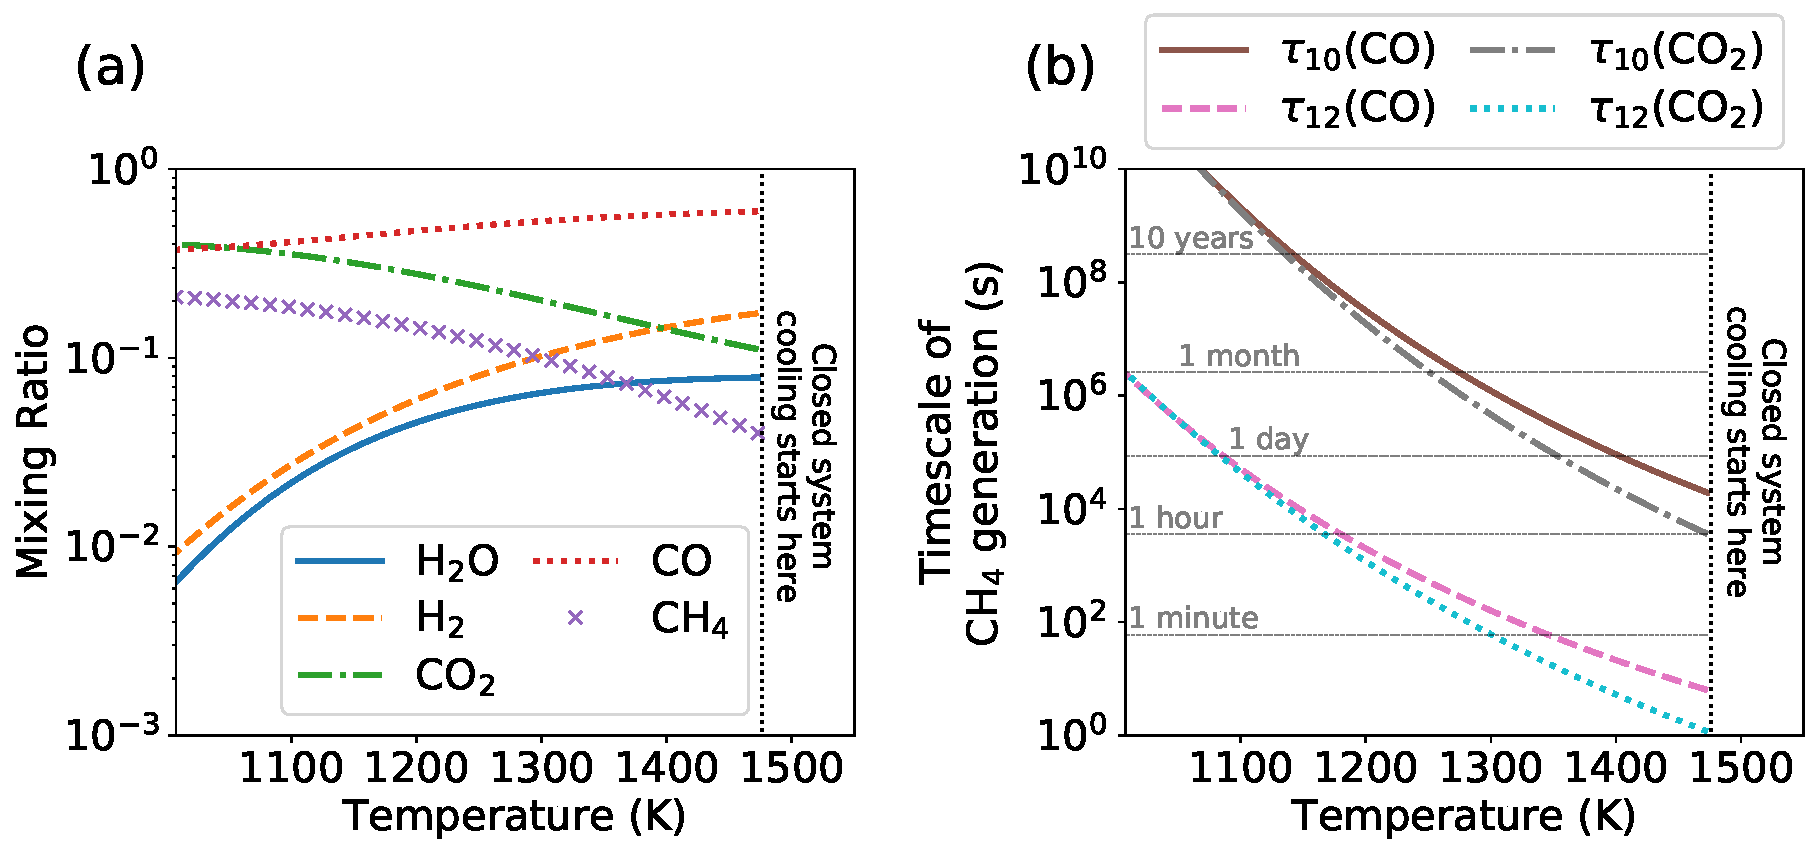
\includegraphics[width=\textwidth]{tex/3methane/figures/kinetics.pdf}
    \caption{(a) Equilibrium composition as a function of temperature for a submarine volcanic gas which is cooled as a closed system and (b) timescales of CH$_4$ formation during closed system cooling. Timescales of volcanic gas cooling are not shown or calculated.}
    \label{fig:kinetics}
\end{figure}

\begin{table}[hbt!]
  \caption{Boundary conditions for photochemical modeling}
  \label{tab:photochem_model}
  \centering
  \begin{tabularx}{\textwidth}{l c c c}
  \hline \hline
  Chemical Species & Deposition Velocity (cm s$^{-1}$) & Mixing Ratio & Flux (molecules cm$^{-2}$ s$^{-1}$)   \\
  \hline
  $\mathrm{O}$ & 1 & ... & ... \\
  $\mathrm{O_2}$ & $1.4\times10^{-4}$ & ... & ... \\
  $\mathrm{H_2O}$ & 0 & ... & ... \\
  $\mathrm{H}$ & 1 & ... & ... \\
  $\mathrm{OH}$ & 1 & ... & ... \\
  $\mathrm{HO_2}$ & 1 & ... & ... \\
  $\mathrm{H_2O_2}$ & $2\times10^{-1}$ & ... & ... \\
  $\mathrm{H_2}$ & 0 & ... & $5.9F_\mathrm{CH_4}$ \\
  $\mathrm{CO}$ & $1\times10^{-8}$ & ... & $1.7F_\mathrm{CH_4}$ \\
  $\mathrm{HCO}$ & 1 & ... & ... \\
  $\mathrm{H_2CO}$ & $2\times10^{-1}$ & ... & ... \\
  $\mathrm{CH_4}$ & 0 & ... & variable \\
  $\mathrm{CH_3}$ & 1 & ... & ... \\
  $\mathrm{C_2H_6}$ & 0 & ... & ... \\
  $\mathrm{NO}$ & $3\times10^{-4}$ & ... & ... \\
  $\mathrm{NO_2}$ & $3\times10^{-3}$ & ... & ... \\
  $\mathrm{HNO}$ & 1 & ... & ... \\
  $\mathrm{O_3}$ & $7\times10^{-2}$ & ... & ... \\
  $\mathrm{HNO_3}$ & $2\times10^{-1}$ & ... & ... \\
  $\mathrm{H_2S}$ & $2\times10^{-2}$ & ... & $0.1F_\mathrm{CH_4}$ \\
  $\mathrm{SO_3}$ & 0 & ... & ... \\
  $\mathrm{S_2}$ & 0 & ... & ... \\
  $\mathrm{HSO}$ & 1 & ... & ... \\
  $\mathrm{H_2SO_4}$ & 1 & ... & ... \\
  $\mathrm{SO_2}$ & 1 & ... & $0.1F_\mathrm{CH_4}$ \\
  $\mathrm{SO}$ & 0 & ... & ... \\
  $\mathrm{SO_4}$ aerosol & $1\times10^{-2}$ & ... & ... \\
  $\mathrm{S_8}$ aerosol & $1\times10^{-2}$ & ... & ... \\
  hydrocarbon aerosol & $1\times10^{-2}$ & ... & ... \\
  $\mathrm{CO_2}$ & ... & variable & ... \\
  $\mathrm{N_2}$ & ... & 0.8 & ... \\
  \hline
  \multicolumn{4}{>{\raggedright\arraybackslash}p{\textwidth}}{Notes. Species included in the photochemical scheme with a deposition velocity and flux of 0 include N, $\mathrm{C_3H_2}$, C$_3$H$_3$, CH$_3$C$_2$H, CH$_2$CCH$_2$, C$_3$H$_5$, C$_2$H$_5$CHO, C$_3$H$_6$, C$_3$H$_7$, C$_3$H$_8$, C$_2$H$_4$OH, C$_2$H$_2$OH, C$_2$H$_5$, C$_2$H$_4$, CH, CH$_3$O$_2$, CH$_3$O, CH$_2$CO, CH$_3$CO, CH$_3$CHO, C$_2$H$_2$, (CH$_2$)$_3$, C$_2$H, C$_2$, C$_2$H$_3$, HCS, CS$_2$, CS, OCS, S, and HS. Here, deposition velocities follow those used by \citet{Schwieterman_2019}.} 
  \end{tabularx}
\end{table}

Suppose that the CH$_4$ quench temperature was instead 1000 K. In this case, the CH$_4$ content of the gas would be increased by about a factor of 5 (Figure \ref{fig:kinetics}a). There are two ways that a $\sim$1000 K CH$_4$ quench is possible. First, gas cooling could occur on timescales of months rather than seconds. According to Figure \ref{fig:kinetics}b, month-long gas cooling should quench CH$_4$ by 1000 K. Second, catalysts could dramatically speed up the reactions creating CH$_4$, which might allow for quench temperatures near 1000 K for even gas cooling timescales of seconds. In the following two paragraphs we show that either of these scenario would not significantly change our results. 

To demonstrate that re-equilibration of gases to feasible lower temperatures does not change our conclusions, assuming low CH$_4$ quench temperatures can be achieved, we perform another Monte-Carlo simulation identical to the one described in Section \ref{sec:monte} except we account for closed system cooling of volcanic gases. In the Monte-Carlo simulation we first calculate gas composition using our outgassing model (Section \ref{sec:volcmodel}), then we re-equilibrate this gas mixture to the uniformly sampled gas equilibrium temperature between 800 and 1500 K. This range of gas equilibrium temperatures is the range observed in Earth's volcanic gases \citep{Moussallam_2019}. In cases where the randomly drawn gas equilibrium temperature is higher than the magma temperature, we assume no closed system cooling occurs.

Figure \ref{fig:CH4_closed} is identical to Figure \ref{fig:CH4}c and \ref{fig:CH4}d, except Figure \ref{fig:CH4_closed} accounts for closed system cooling of gases. Closed system cooling allows more CH$_4$ production on average, but still only 0.3\% and 0.1\% of calculations for ocean worlds or earth-like worlds respectively produce more than 10 Tmol CH$_4$/yr. The probability of volcanic CH$_4$ fluxes being comparable to modern Earth's biological flux (30 Tmol/yr) is still low.

\begin{figure*}
    \centering
    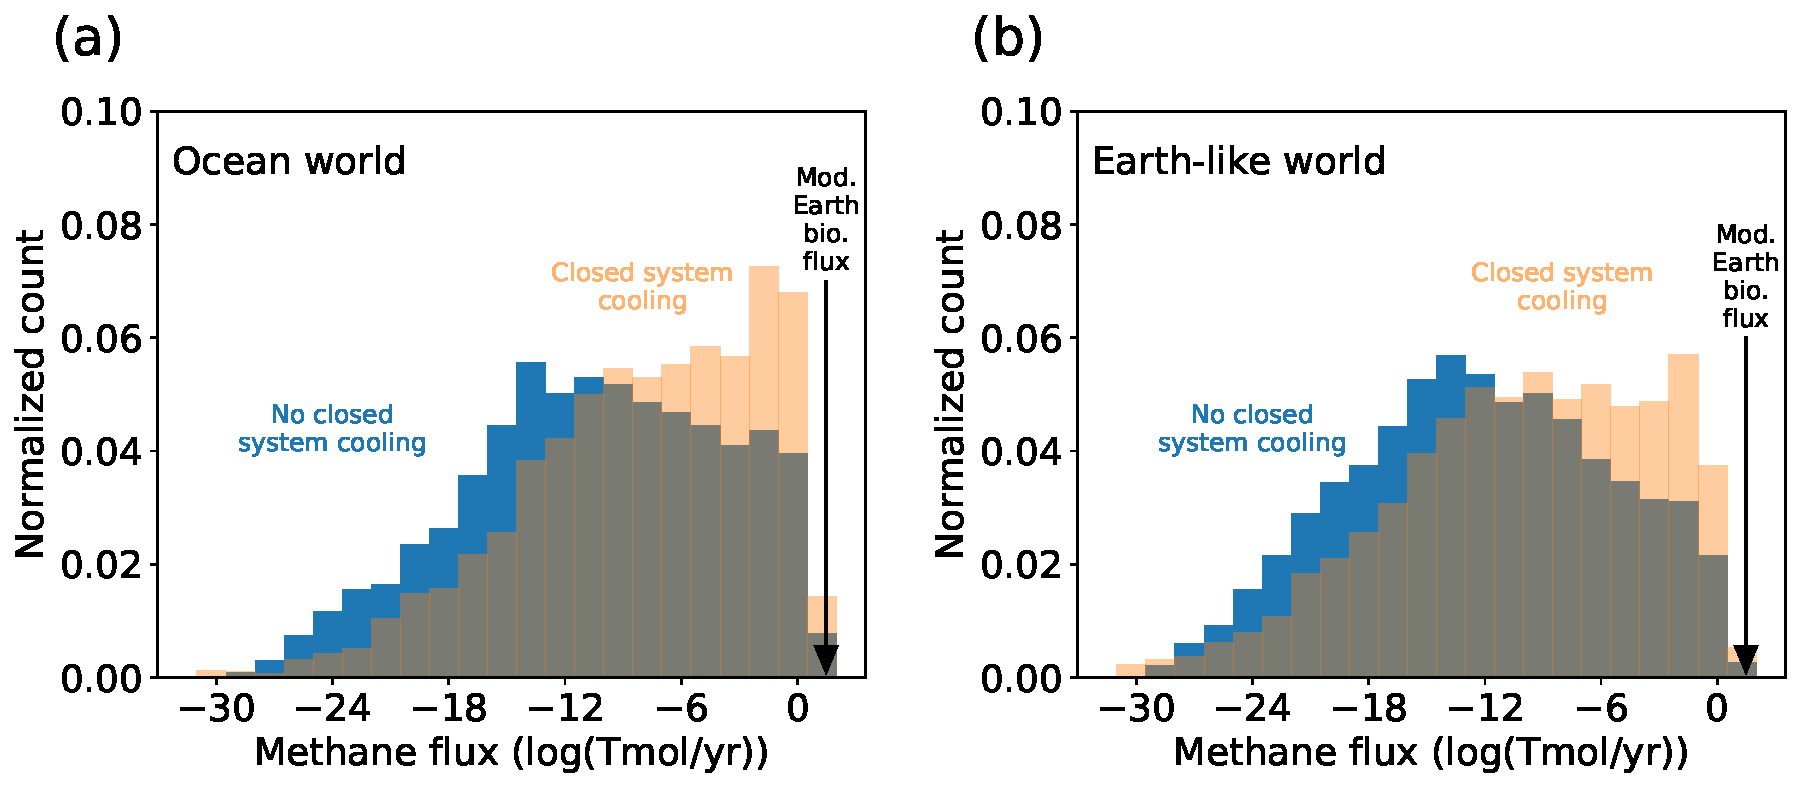
\includegraphics[width=\textwidth]{tex/3methane/figures/CH4_prod_closedsystem.pdf}
    \caption{The blue histograms in (a) and (b) are identical to Figure \ref{fig:CH4}c and \ref{fig:CH4}d, and orange histograms are identical Monte Carlo simulations except they account for the closed system cooling of volcanic gases to equilibrium temperatures observed on Earth (800 to 1500 K). To calculate CH$_4$ fluxes, we used modern Earth's magma production rate.}
    \label{fig:CH4_closed}
\end{figure*}

In summary, changes in gas chemistry during cooling might cause our speciation model to under-predict the CH$_4$ produced by an amount that does not change our conclusions significantly. Further consideration of the kinetics of CH$_4$ generation in volcanic gases is beyond the scope of this paper.

\subsection{Photochemical model boundary conditions} \label{sec:photo_boundary_cond}

Table \ref{tab:photochem_model} shows boundary conditions used for the \textit{Atmos} photochemical model. We used the same H$_2$O and temperature profile as \citet{Kharecha_2005} for all simulations. The version of Atmos that we used has updated rate constants and H$_2$O cross sections following \citet{Ranjan_2020}.

Every simulation for planets orbiting the Sun uses a solar spectrum at 2.7 Ga calculated using methods described in \citet{Claire_2012}, although our results are not sensitive to age of the Sun. For planets orbiting a M8V star, we use estimates of TRAPPIST-1's spectrum derived by \citet{Lincowski_2018}, scaled so that the solar constant of the planet is 0.822 relative to modern Earth's. We use this solar constant because it places the simulated planet at the same relative distance from the inner edge of the habitable zone as Earth today \citep{Kopparapu_2013}.

All of our models include the modern production rate of NO from lightning.